\documentclass[a4paper,14pt]{extarticle}

\usepackage{cmap}

\usepackage[T2A, T1]{fontenc}
\usepackage[utf8]{inputenc}
\usepackage[english,russian]{babel}

\usepackage{geometry}
\geometry{a4paper,top=2cm,bottom=2cm,left=3cm,right=2cm}

\renewcommand{\rmdefault}{Tempora-TLF}

\usepackage{textcase}
\usepackage{anyfontsize}

\linespread{1.213}

\usepackage{indentfirst}
\setlength\parindent{1.25cm}

\usepackage{amsmath,amssymb,amsthm,latexsym,amsfonts}
\usepackage[unicode,hidelinks]{hyperref}

\usepackage{textcomp}
\usepackage{imakeidx}
\usepackage{hyperref}
\frenchspacing
\usepackage{mathtools}
\usepackage{graphicx}
\usepackage{float}
\usepackage{caption}
\usepackage{subcaption}
\usepackage{tabularx}
\usepackage{multirow}
\usepackage{array}

\usepackage{tabularray}
\UseTblrLibrary{booktabs}

\graphicspath{{images/}}

\usepackage[hidelinks]{hyperref}

\usepackage[justification=centering]{caption}
\DeclareCaptionLabelSeparator{point}{. }
\captionsetup{labelsep=point}

\usepackage[raggedright]{titlesec}
\titleformat{\section}[block]{\Large\bfseries\filcenter}{}{0em}{}
\titlespacing{\section}{0pt}{18pt}{18pt}
\titleformat{\subsection}[block]{\large\bfseries\filcenter}{}{0em}{}
\titlespacing{\subsection}{0pt}{18pt}{18pt}

\newcommand{\norm}[1]{\left\lVert#1\right\rVert}

\usepackage[dvipsnames]{xcolor}
\definecolor{mygreen}{RGB}{50, 203, 0}
\definecolor{myred}{RGB}{254, 0, 0}
\definecolor{myblue}{RGB}{49, 102, 255}

\usepackage{microtype}
\usepackage{ragged2e}

\justifying
\sloppy
\tolerance=500
\hyphenpenalty=10000
\emergencystretch=3em

\begin{document}

\begin{titlepage}

\newpage

\begin{center}
Филиал Московского Государственного Университета

имени М.В. Ломоносова в городе Ташкенте

Факультет прикладной математики и информатики

Кафедра прикладной математики и информатики

\hrulefill
\end{center}

\vspace{3em}

\begin{center}
\large Иничкина Наталья Сергеевна
\end{center}

\vspace{2em}

\begin{center}
\textsc{\textbf{ВЫПУСКНАЯ КВАЛИФИКАЦИОННАЯ РАБОТА}}
\end{center}

\begin{center}
\textsc{\textbf{на тему: <<Применение нейросетевых алгоритмов в задаче трекинга объектов на видео при наблюдении с беспилотных летательных аппаратов>> \\ по направлению 01.03.02 <<Прикладная математика и информатика>>}}
\end{center}

\vspace{3em}

\begin{flushleft}
ВКР рассмотрена и рекомендована к защите\\
зав. кафедрой <<ПМиИ>>, д.ф.-м.н., профессор
\hrulefill \ Гасанов Э.Э.
\end{flushleft}

\vspace{0.1em}

\begin{flushleft}
Научный руководитель\\
к.ф.-м.н., н. с.
\hrulefill \ Половников В.С.
\end{flushleft}

\vspace{0.1em}

\begin{flushright}
<<\underline{\hspace{1cm}}>> \underline{\hspace{3cm}} 2023 г.
\end{flushright}

\vspace{\fill}

\begin{center}
Ташкент 2023
\end{center}

\end{titlepage}

\thispagestyle{empty}

\begin{abstract}

    В данной работе рассматривается задача трекинга множества объектов на видео при наблюдении с беспилотных летательных аппаратов. Представлено решение проблемы несбалансированности классов для датасета VisDrone. Реализована модель YOLOv5-StrongSORT-GSI. Проведено сравнение полученной модели и встроенных алгоритмов трекинга новейшей модели YOLOv8, показавшее более высокую точность трекинга первой из них.

    \vspace{0.2cm}

    \textbf{Ключевые слова:} трекинг множества объектов, YOLO, VisDrone, проблема несбалансированности классов, UAVDT, StrongSORT
    
\end{abstract}

\renewcommand{\abstractname}{Abstract}

\begin{abstract}

    This paper considers the task of multiple object tracking on video from unmanned aerial vehicles. A solution to the class imbalance problem for the VisDrone dataset is presented. The YOLOv5-StrongSORT-GSI model is implemented. A comparison between the obtained model and the newest YOLOv8 integrated tracking algorithms is performed, which results in higher tracking accuracy of the first one.

    \vspace{0.2cm}

    \textbf{Keywords:} multiple object tracking, YOLO, VisDrone, class imbalance problem, UAVDT, StrongSORT
    
\end{abstract}


\tableofcontents
\setcounter{page}{3}

\section*{Введение}
\addcontentsline{toc}{section}{Введение}

В современном мире беспилотные летательные аппараты стали неотъемлемой частью многих сфер человеческой деятельности благодаря своей универсальности и эффективности в применении \cite{1-1}, что позволило им стать мощным инструментом в различных прикладных задачах, таких как картография \cite{1-2}, система предупреждения лесных пожаров \cite{1-3}, система оперативного спасения людей \cite{1-4} и содействие в контроле чрезвычайных ситуаций \cite{1-5}.

Однако использованию беспилотных летательных аппаратов в вышеперечисленных областях сопутствует множество проблем, нестандартных для работы с видеоматериалами, полученными с помощью статичных камер видеонаблюдения, таких как вызванное движением камер размытие, помехи в сигналах передачи, переменные погодные условия и варьирующиеся размеры объектов, связанные с изменением высоты точки обзора \cite{1-6}.

В целях полного раскрытия потенциала использования беспилотных летательных аппаратов и расширения сфер их применения разрабатывается множество алгоритмов и моделей в области искусственного интеллекта \cite{1-7}, активно использующегося в задачах поиска, классификации и трекинга объектов как на записях с камер, так и в условиях реального времени.

Первоначальным этапом трекинга является детектирование и классификация, заключающиеся в выделении на каждом отдельном кадре объектов, например, ограничивающими рамками, и определении классов, к которым они принадлежат. Некоторыми из известных и пользующихся популярностью решений данной задачи являются R-CNN \cite{1-8} и версия для более быстрых вычислений FAST R-CNN \cite{1-9}, их модификация FASTER R-CNN \cite{1-10}, использующая для генерации областей возможного наличия объектов специальную нейронную сеть RPN (Region Proposal Network), Mask R-CNN \cite{1-11} и TensorMask \cite{1-12}, позволяющие решать задачу сегментации, а также RetinaNet \cite{1-13} и YOLO \cite{1-14}, отличительной особенностью которых является их одностадийная архитектура.

Следующим этапом данной задачи служат алгоритмы трекинга, позволяющие сопоставлять объекты и определять взаимосвязь их расположений на соседних кадрах из общей последовательности, что позволяет устанавливать для каждого объекта на видео его уникальный идентификационный номер, что, в свою очередь, делает возможным подсчет объектов на видео. Возникающая проблема сопоставления траекторий таких объектов может решаться применением алгоритмов трекинга, таких как SORT \cite{1-15} и его улучшения при помощи реидентифицации объектов по их внешнему виду DeepSORT \cite{1-16}, TransMOT \cite{1-17}, представляющим упорядоченные траектории всех отслеживаемых объектов в виде серии разреженных взвешенных графов, построенных с использованием пространственных отношений между целями, а также StrongSORT \cite{1-18} и ByteTrack \cite{1-19}.

Дополнительным этапом может служить постобработка, позволяющая улучшить работу алгоритма трекинга и повысить точность результатов, например, при помощи сглаживания траекторий и дополнения пропущенных моментов движения. Примерами такого механизма улучшения трекинга являются фильтр Калмана \cite{1-20}, фильтр частиц \cite{1-21} и сегментация \cite{1-22}.

\section*{Постановка задачи}
\addcontentsline{toc}{section}{Постановка задачи}

Целью данной работы является реализация трекинга множества объектов на видео с помощью нейронных сетей и сравнительный анализ с известными решениями.

Работа включает в себя обучение нейронной сети семейства YOLOv5 \cite{2-1} с помощью датасета VisDrone \cite{2-2}, размещенного командой AISKYEYE в рамках Vision Meets Drones: A Challenge \cite{2-3}, и датасета UAVDT, представленного в статье, опубликованной в материалах семинара IEEE Conference on Computer Vision and Pattern Recognition Workshops \cite{2-4} в 2018 году, прошедших предварительную обработку, применение алгоритма трекинга StrongSORT \cite{2-5} и реализацию постобработки полученных результатов с помощью алгоритма, осуществляющего линейную интерполяцию \cite{2-6} и гауссовское сглаживание \cite{2-7}, а также оценку точности полученной модели и сравнение с существующими результатами.

\section{Данные}

\subsection{VisDrone}

VisDrone -- набор из 288 видео, сформированный из 261,908 кадров и 10,209 статических изображений, полученных с помощью различных камер с беспилотных летательных аппаратов в городах Китая при разных погодных условиях и варьирующейся освещенности, с различным количеством объектов и их плотностью в кадре, с разных ракурсов и позиций в воздушном пространстве, как показано на Рис. \ref{img:3-1}.

\vspace{0.5cm}

\begin{figure}[ht]
    \centering
    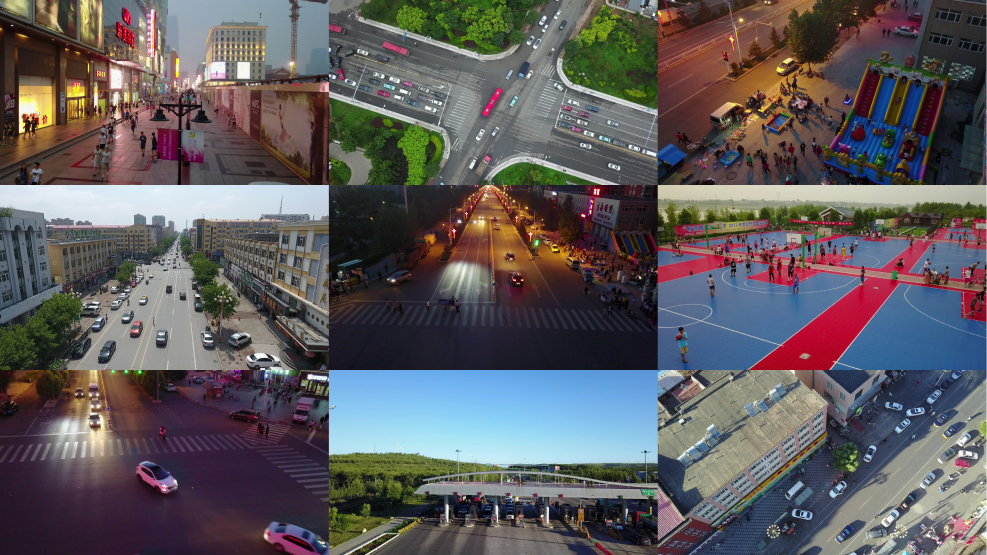
\includegraphics[width=0.85\textwidth]{3-1}
    \caption{Пример выборки кадров из VisDrone}
    \label{img:3-1}
\end{figure}

Датасет был создан командой AISKYEYE из лаборатории машинного обучения и сбора данных Тяньцзиньского университета в Китае с целью формирования базы для проведения оценки моделей и исследования алгоритмов визуального анализа, связанных с беспилотными летательными аппаратами. Все полученные материалы были вручную аннотированы при помощи 2.6 миллиона ограничивающих рамок, кадры с примерами которых представлены на Рис. \ref{img:3-2}.

\begin{figure}[ht]
    \centering
    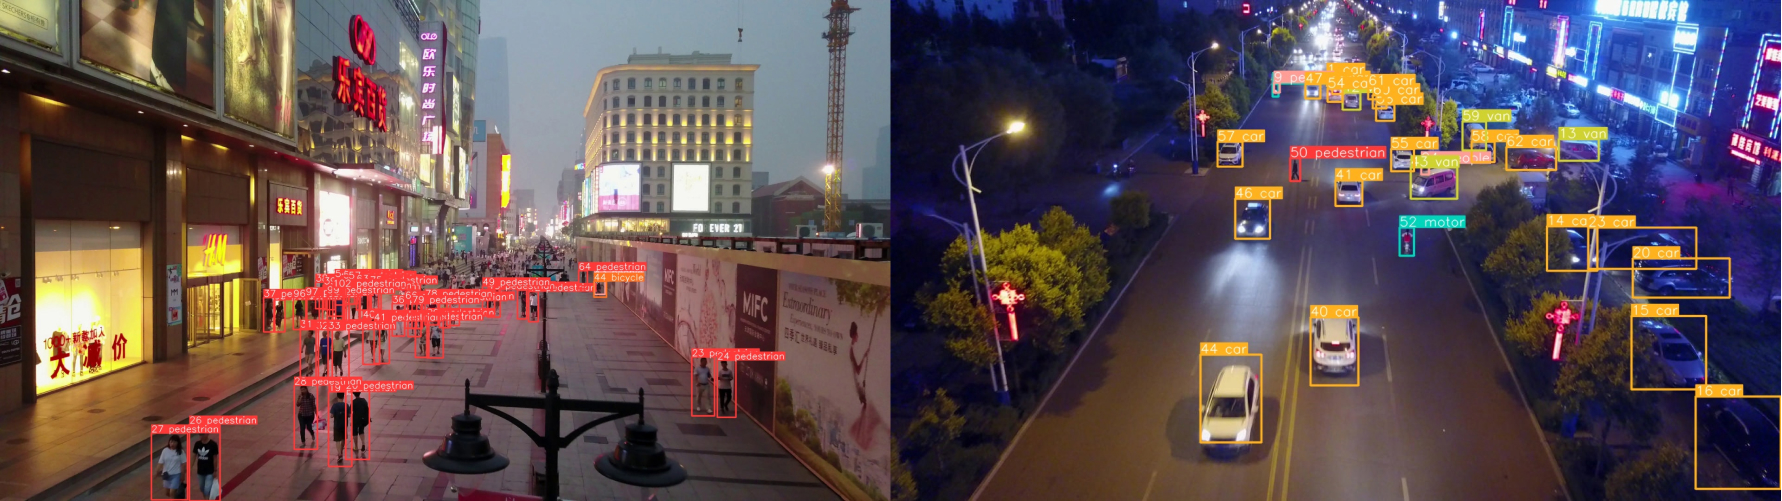
\includegraphics[width=0.85\textwidth]{3-2}
    \caption{Пример аннотированных кадров VisDrone}
    \label{img:3-2}
\end{figure}

Весь датасет подразделяется на 5 задач: детектирование объектов на изображениях, детектирование объектов на видео, трекинг одного объекта, трекинг множества объектов и подсчет количества людей в толпе. В датасете представлено 10 классов: pedestrian, person, car, van, bus, truck, motor, bicycle, awning-tricycle и tricycle.
Используемая в данной работе часть датасета -- VisDrone-MOT2019 -- состоит из 79 видеорядов из 33,366 кадров суммарно, из которых train -- 56 видеорядов из 24,198 кадров, val -- 7 видеорядов из 2,846 кадров, test -- 16 видеорядов из 6,322 кадров.

Следует заметить, что в датасете присутствует значительно выраженная несбалансированность классов, создающая видимые затруднения в классификации объектов, что наглядно показано на Рис. \ref{img:3-3}. Наиболее представленным является класс car, объем которого почти в 2.5 раза превышает второй по распространенности класс pedestrian и в 50 раз класс bus.

\begin{figure}[ht]
    \centering
    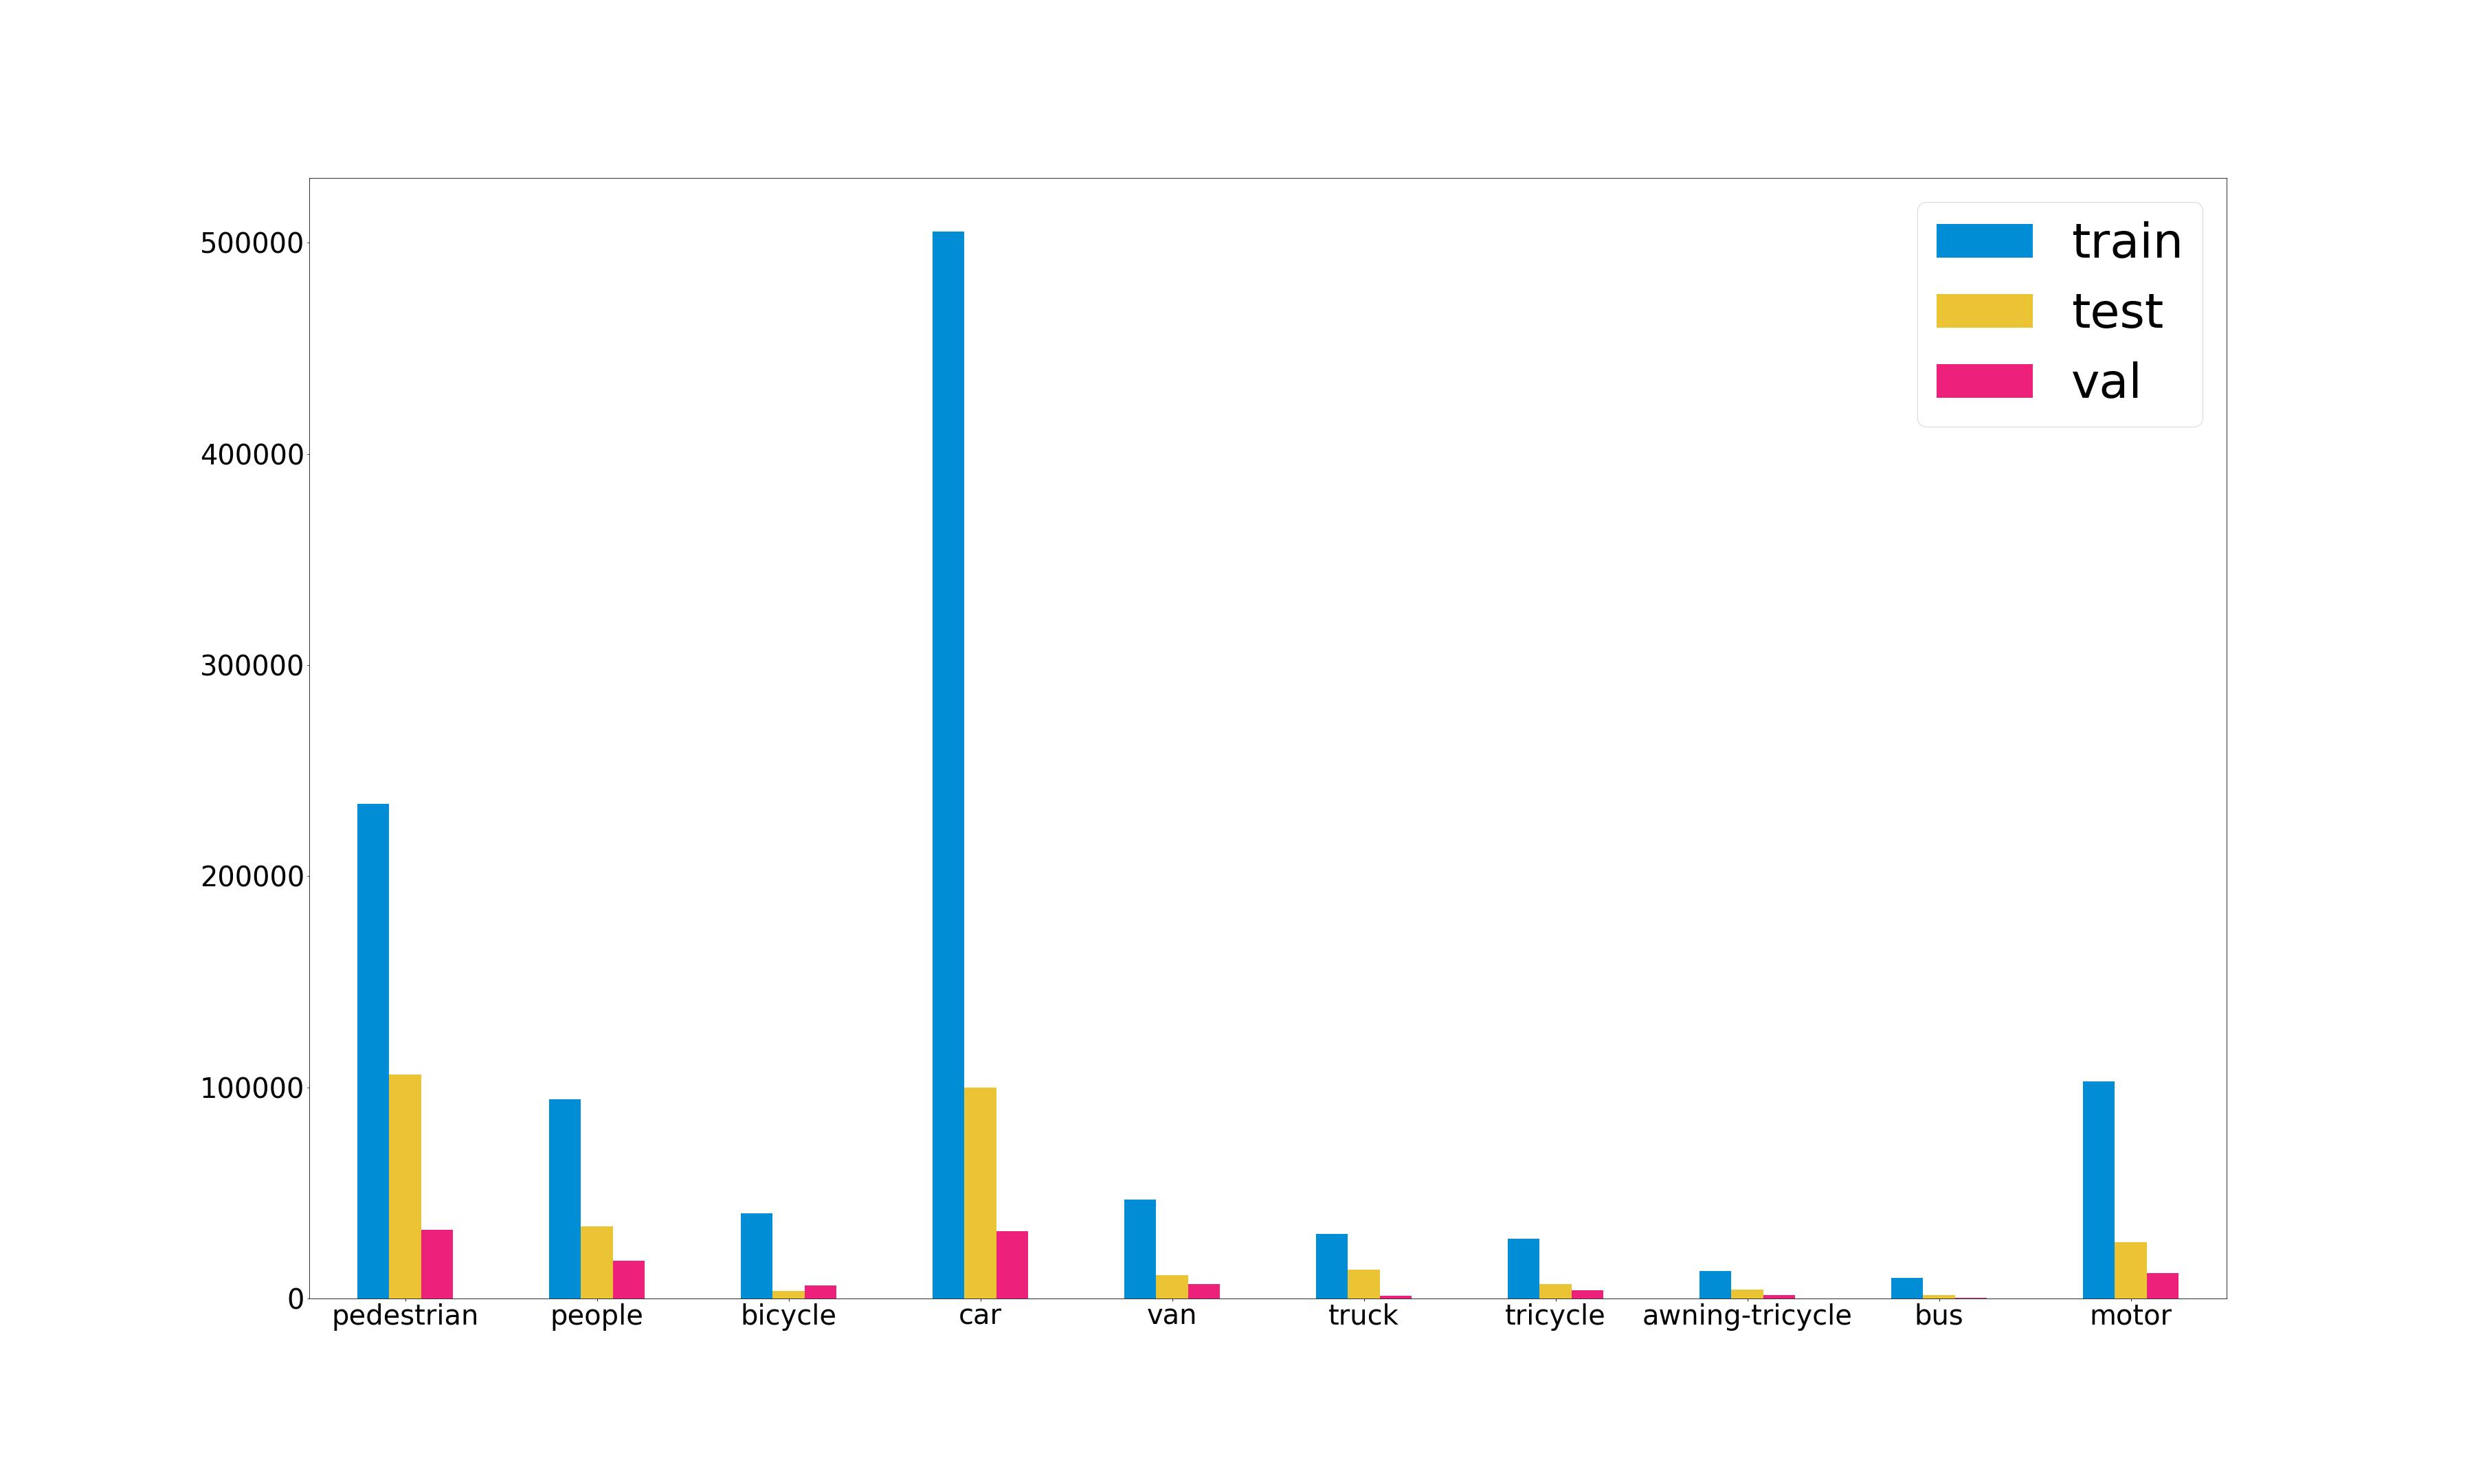
\includegraphics[width=0.85\textwidth]{3-3}
    \caption{Распределение объектов по классам в VisDrone-MOT2019}
    \label{img:3-3}
\end{figure}

\subsection{UAVDT}

UAVDT (Unmanned Aerial Vehicle Benchmark Object Detection and Tracking) \cite{4-1} -- датасет, состоящий из 100 видеопоследовательностей, включающих в себя около 80,000 кадров, отобранных из снятых беспилотными летательными аппаратами 10 часов видео. Данные получены в различных локациях скопления транспорта, таких как площади, магистральные улицы, перекрестки и автостанции, что стало нововведением в датасетах подобной тематики, позволяющем исследовать сложные сценарии автомобильного движения, как можно видеть на Рис. \ref{img:4-1}.

\vspace{0.5cm}

\begin{figure}[ht]
    \centering
    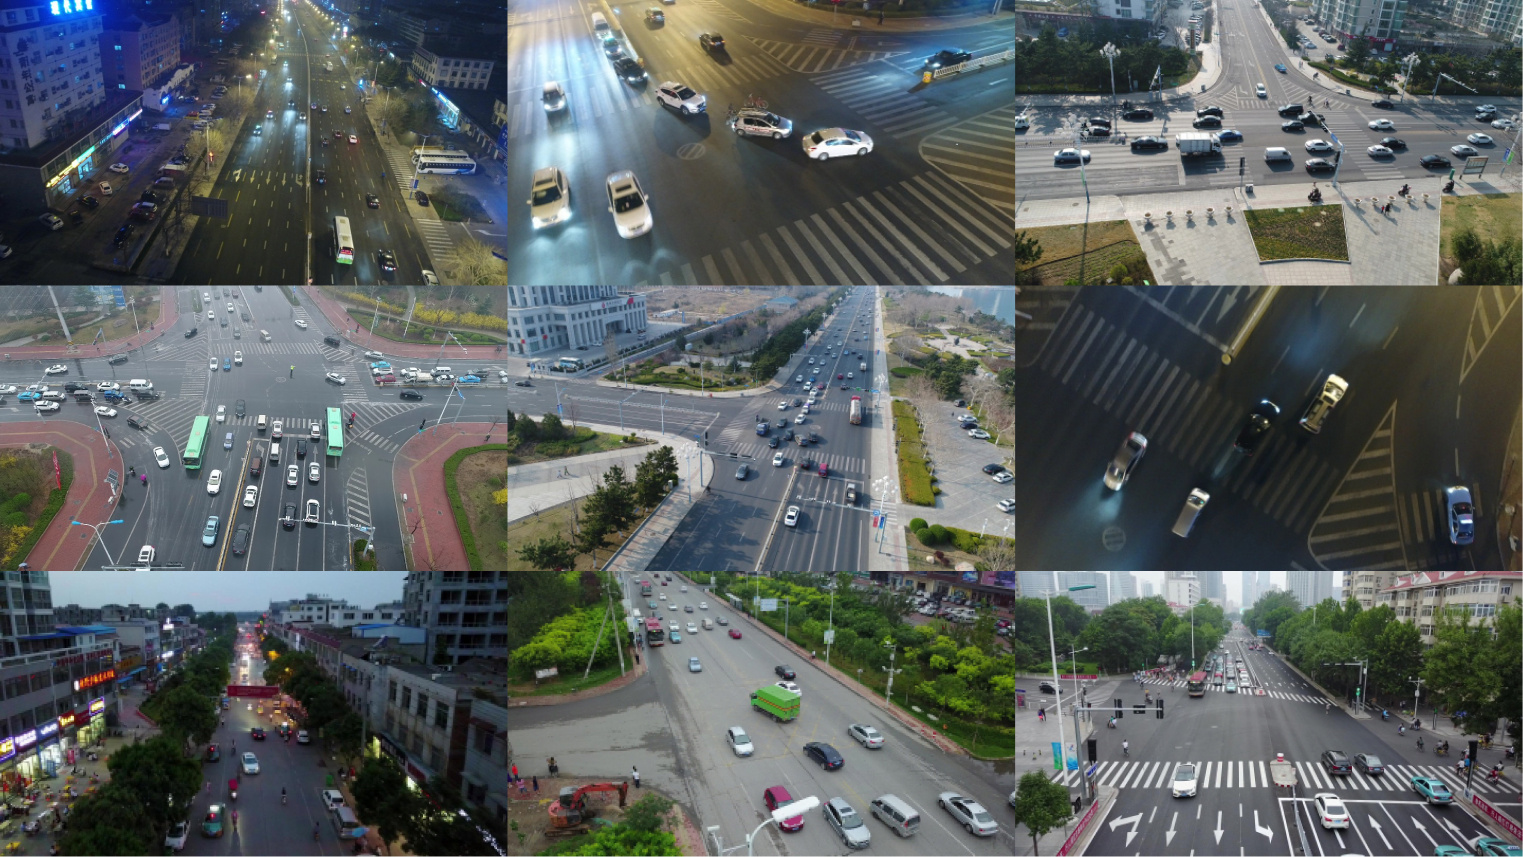
\includegraphics[width=0.85\textwidth]{4-1}
    \caption{Пример выборки кадров из нескольких видео UAVDT}
    \label{img:4-1}
\end{figure}

Датасет был собран командой исследователей из Национального университета Сингапура (NUS) с целью установления стандарта оценки алгоритмов отслеживания объектов в случае сложных сценариев и способствования проведению новых исследований в этой области. Для этого было выполнено аннотирование около 80,000 кадров с помощью 840,000 ограничивающих рамок для 2,700 транспортных средств, как на Рис. \ref{img:4-2}, а также были предоставлены данные о варьирующихся параметрах, таких как высота съемки, погодные условия и точки обзора, краткая информация о которых представлена на Рис. \ref{img:4-3}.

\begin{figure}[ht]
    \centering
    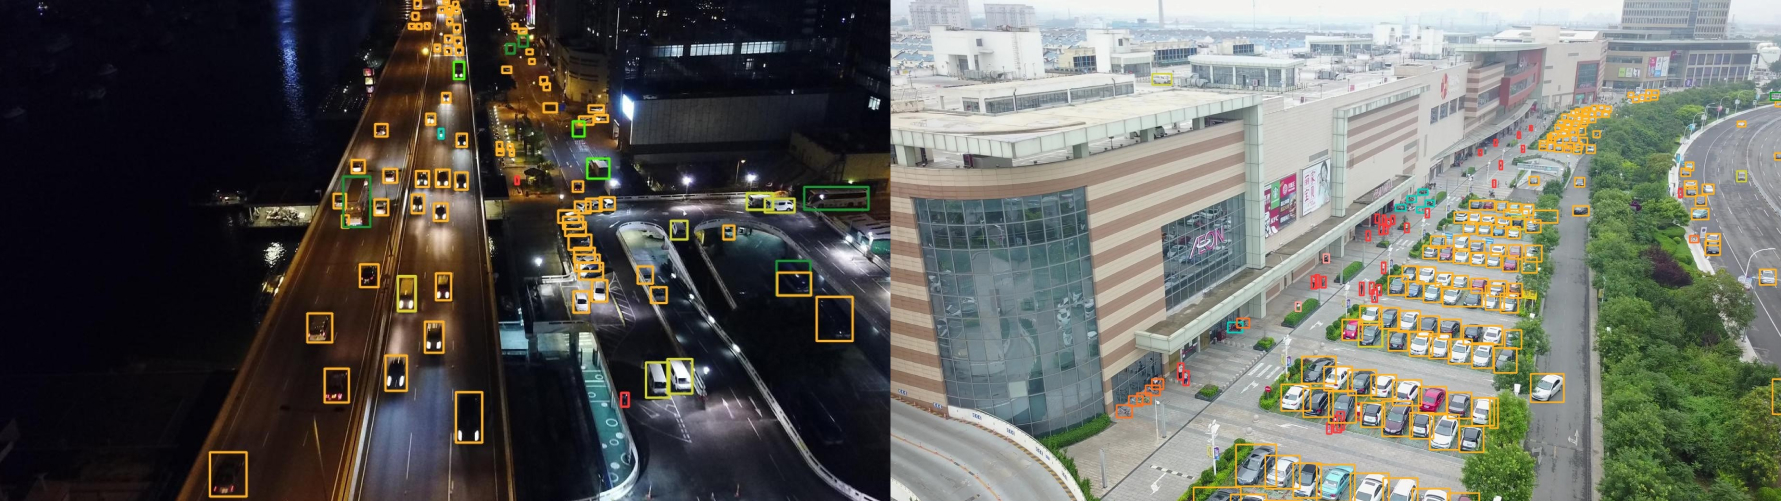
\includegraphics[width=0.85\textwidth]{4-2}
    \caption{Пример аннотированных кадров UAVDT}
    \label{img:4-2}
\end{figure}

\begin{figure}[ht]
    \centering
    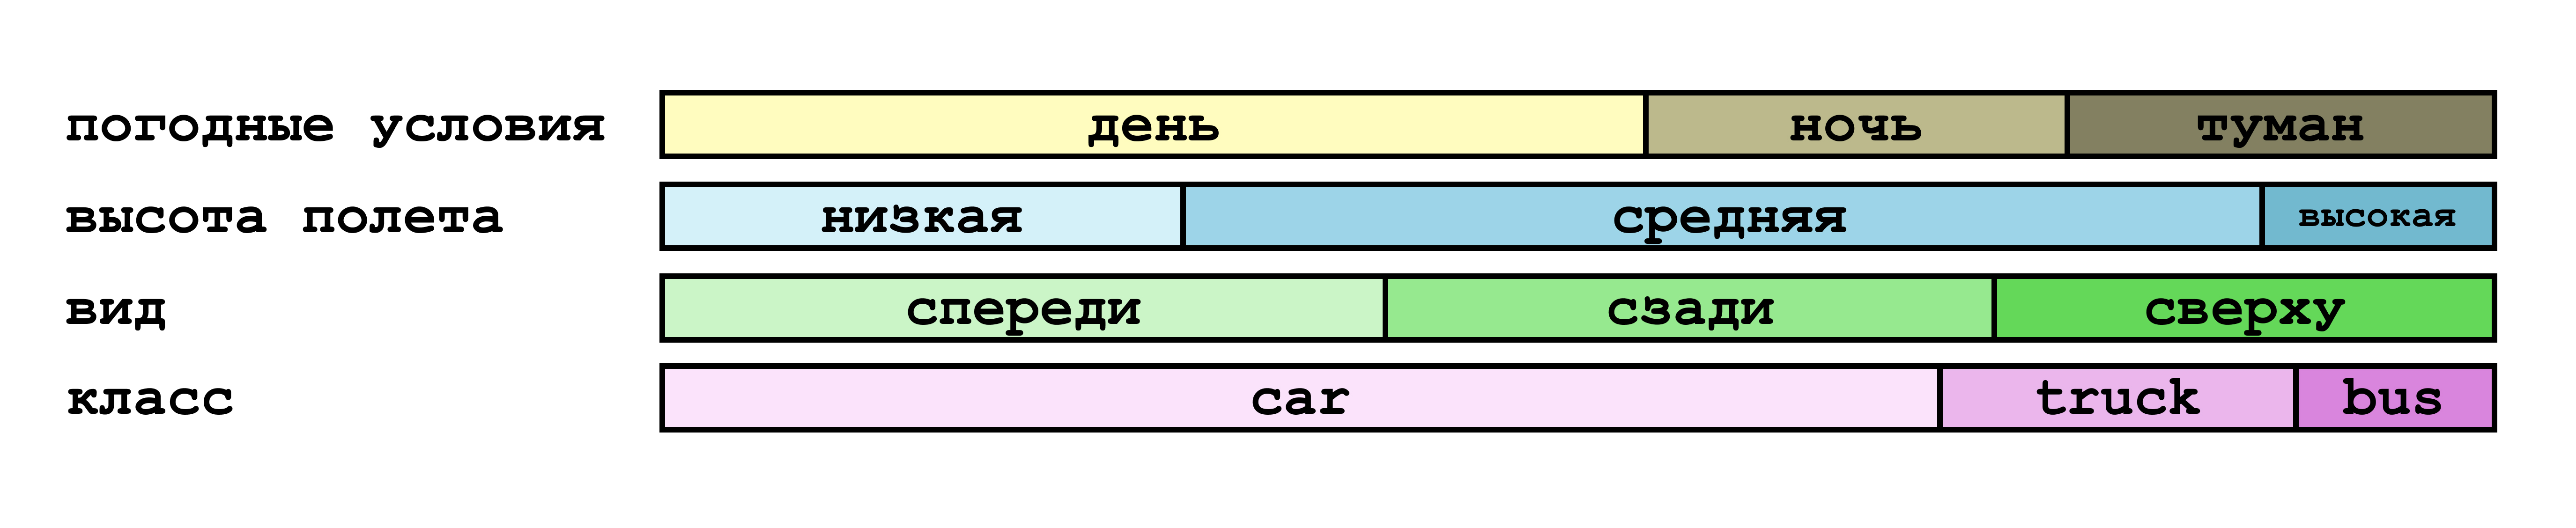
\includegraphics[width=0.85\textwidth]{4-3}
    \caption{Распределение признаков в UAVDT}
    \label{img:4-3}
\end{figure}

Весь датасет подразделяется на 3 задачи: детектирование множества объектов, трекинг одного объекта и трекинг множества объектов. Всего в датасете представлено 3 класса: car, bus и truck, но несмотря на их малое разнообразие, UAVDT обладает более высокой плотностью объектов в кадре, равной 10.52 \cite{4-2}, в сравнении с другими подобными датасетами.

\section{Модели}

\subsection{YOLOv5}

YOLO (You Only Look Once) -- архитектура одностадийной нейронной сети для обнаружения объектов в режиме реального времени, созданная в 2015 году Джозефом Редмоном в университете Вашингтона, главными преимуществами которой являются скорость работы и легковесность.

В 2016 году была выпущена YOLOv2 (YOLO9000) \cite{5-2}, ставшая улучшением оригинальной модели, включив в нее пакетную нормализацию, якорные рамки и кластеры размерности, а также позволившая детектировать объекты из 9000 категорий. YOLOv3 \cite{5-3} была выпущена в 2018 году и усовершенствовала эффективность модели за счет использования более результативной базовой части и добавления пирамид признаков.

В 2020 году была выпущена модель YOLOv4 \cite{5-4}, в которой появился ряд нововведений, таких как использование мозаичной аугментации данных и новая функция потерь. В этом же году команда Ultralytics выпустила реализованную на PyTorch YOLOv5, продемонстрировав резкий скачок в производительности модели.

\begin{figure}[ht]
    \centering
    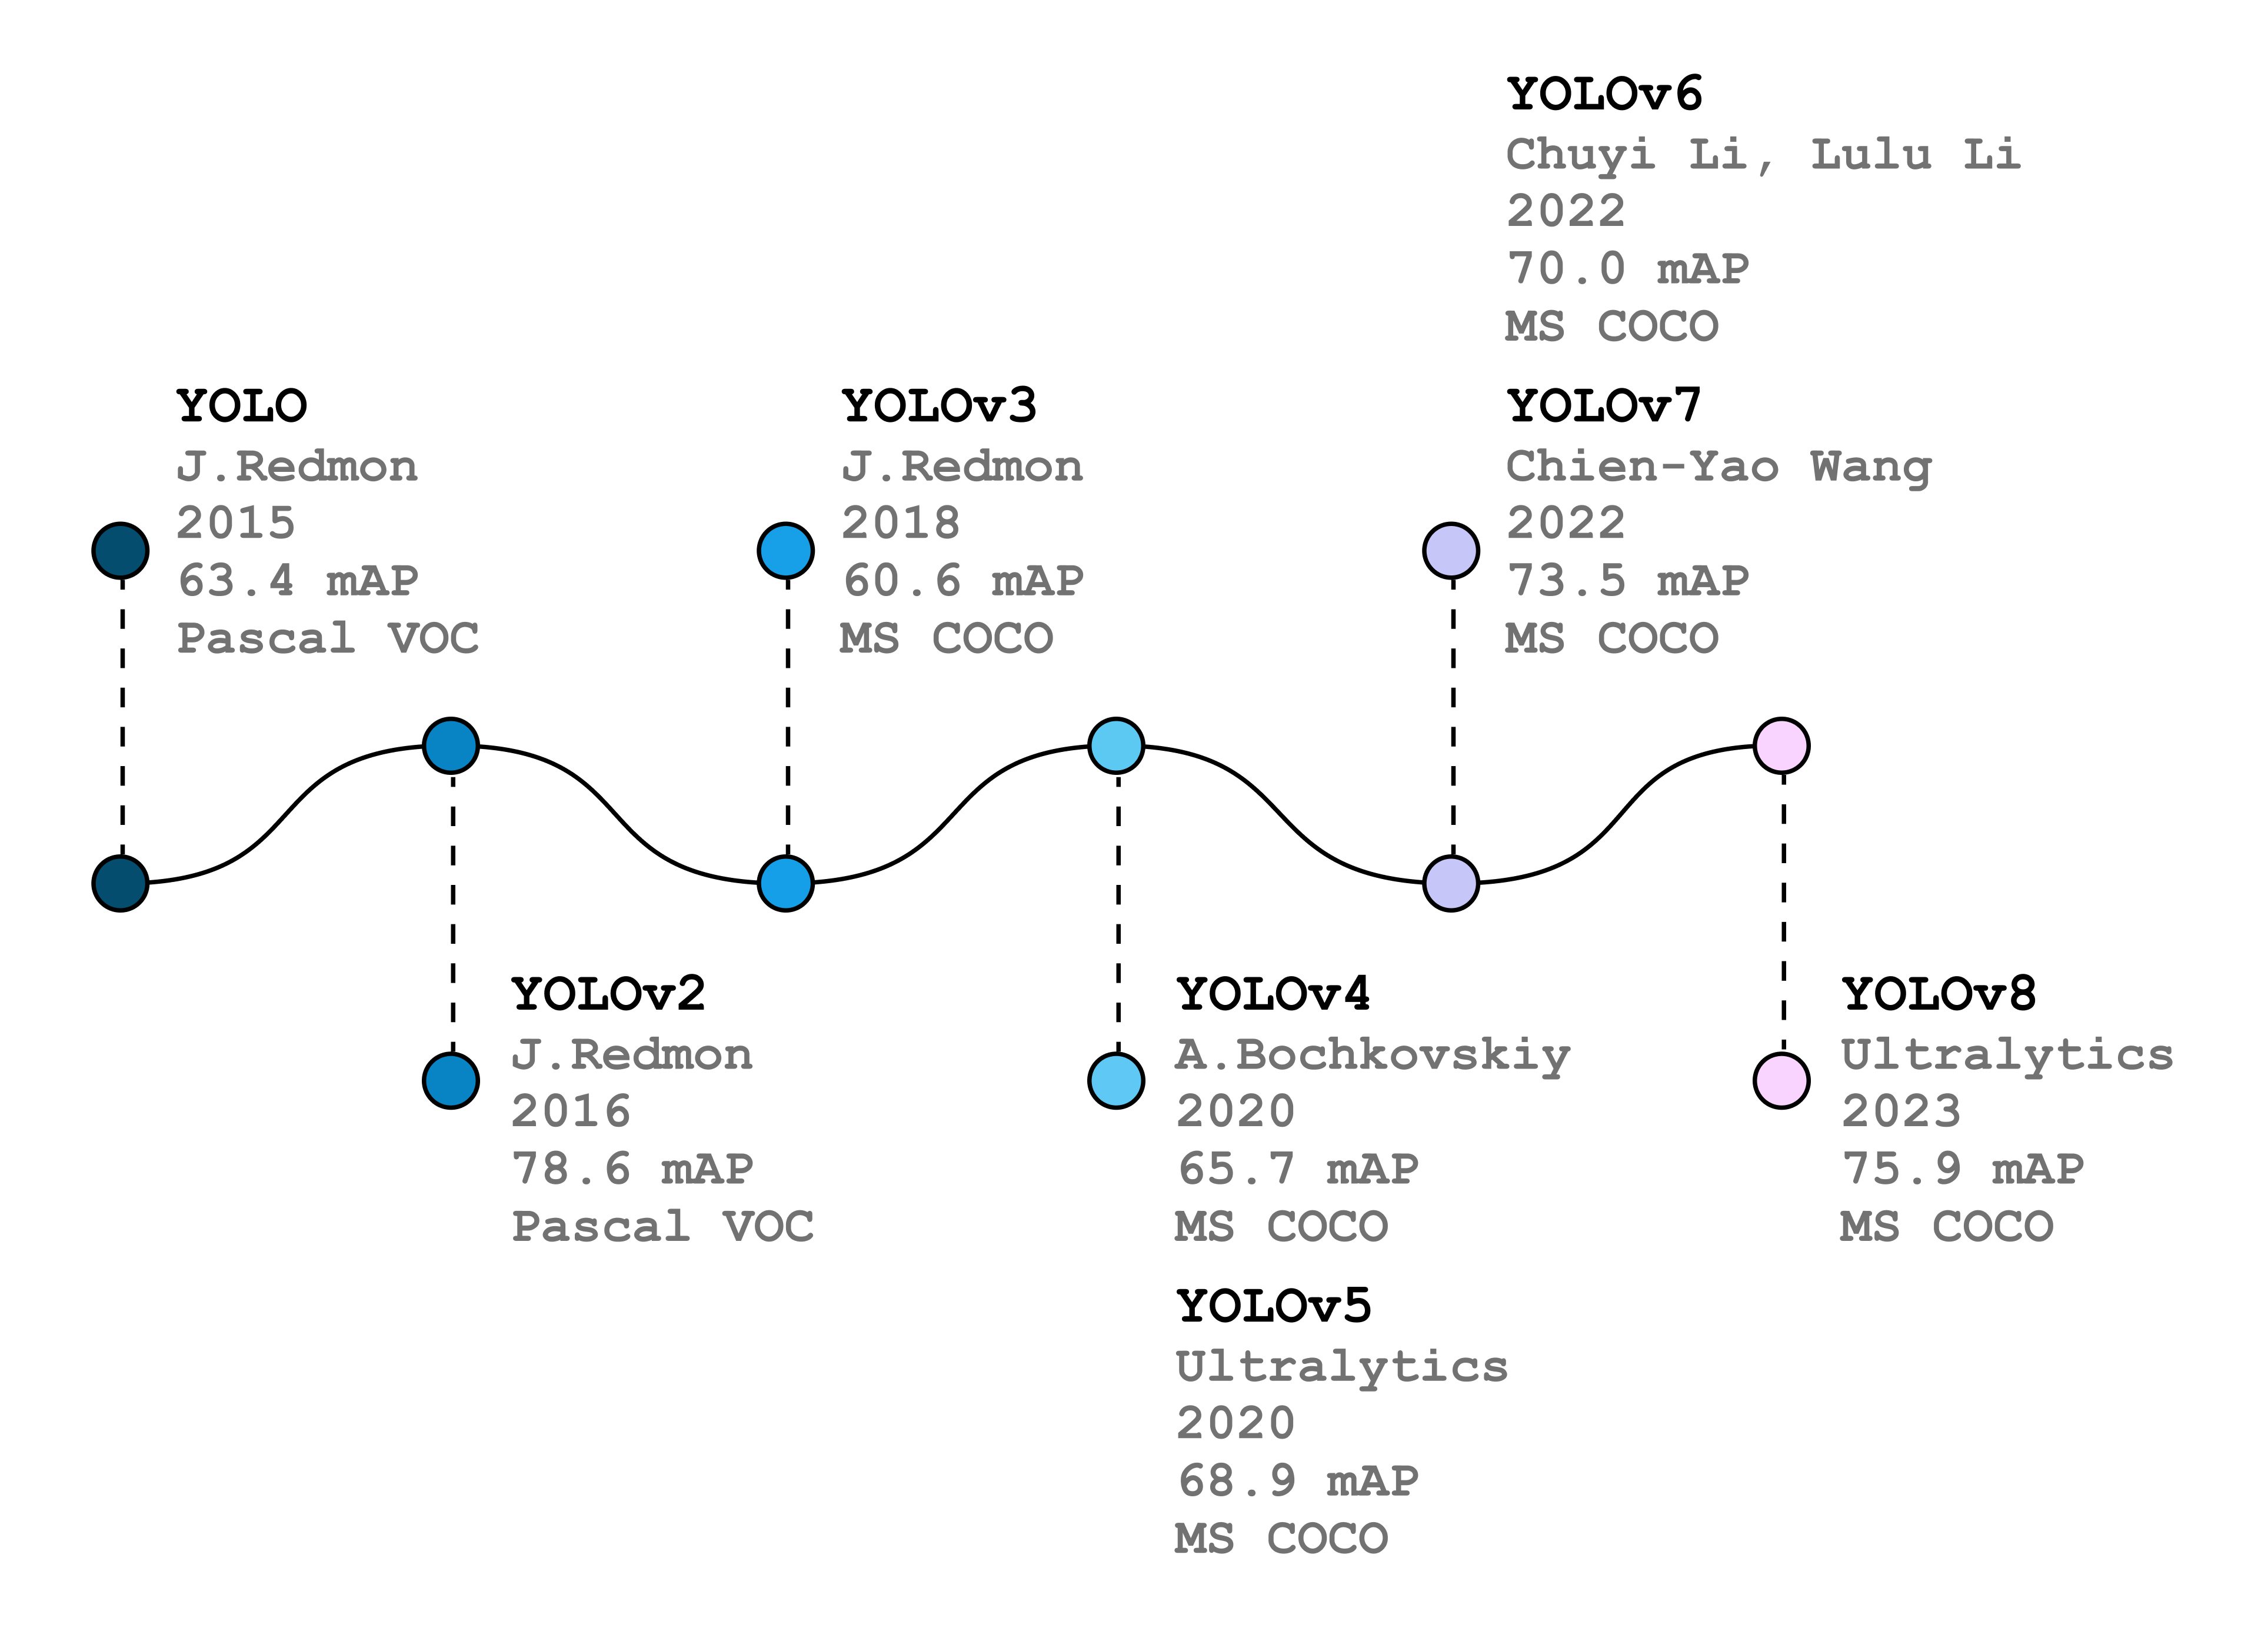
\includegraphics[width=0.85\textwidth]{5-1}
    \caption{История YOLO}
    \label{img:5-1}
\end{figure}

Архитектура используемой одностадийной модели состоит из 3 компонент: Backbone, Neck и Dense Prediction, как показано на Рис. \ref{img:5-1}. Backbone, являющаяся предварительно обученной сетью и используемая для извлечения признаков изображений, способствует уменьшению их разрешения и увеличению пространства признаков. Компонента Neck, используемая для извлечения пирамид признаков, создана для объединения информации с отдельных слоев предыдущих блоков и позволяет модели обобщенно работать с объектами разных размеров и масштабов. Блок Head используется для выполнения операций на заключительном этапе, добавляя якорные рамки к картам признаков и реализуя вывод конечных результатов: классов объектов, оценок точности предсказаний и ограничивающих рамок.

\vspace{0.5cm}

\begin{figure}[ht]
    \centering
    \includegraphics[width=0.85\textwidth]{5-2}
    \caption{Структура одностадийного детектора}
    \label{img:5-2}
\end{figure}

YOLOv5 \cite{5-4} применяет в качестве компоненты Backbone CSP-Darknet53, сверточную нейронную сеть Darknet53, использованную в качестве основы для YOLOv3, к которой применена Cross Stage Partial (CSP). В качестве Neck использованы Spatial Pyramid Pooling (SPP), преимущество которого в значительном увеличении рецептивного поля и выделении наиболее значимых контекстных признаков без снижения скорости работы сети, и Path Aggregation Network (PANet), модифицированная путем добавления BottleNeckCSP в ее архитектуру. Head состоит из трех слоев свертки, которые предсказывают расположение ограничивающих рамок, оценки точности и классы объектов. Схема данной структуры представлена на Рис. \ref{img:5-2}.

\begin{figure}[ht]
    \centering
    \includegraphics[width=0.85\textwidth]{5-3}
    \caption{Схема структуры модели YOLOv5}
    \label{img:5-3}
\end{figure}

По сравнению с предыдущими моделями были представлены новые формулы для вычисления координат ограничивающих рамок, решающие проблему ранних версий с неправильным детектированием объектов в углах и по краям изображений:

\begin{equation}
    b_x = (2 \cdot \sigma(t_x) - 0.5) + c_x
\end{equation}

\begin{equation}
    b_y = (2 \cdot \sigma(t_y) - 0.5) + c_y
\end{equation}

\begin{equation}
    b_w = p_w \cdot (2 \cdot e^{t_w})^2
\end{equation}

\begin{equation}
    b_h = p_h \cdot (2 \cdot e^{t_h})^2
\end{equation}

\vspace{0.5cm}

Концепция работы YOLO, особенность которой состоит в просмотре всего изображения целиком за один раз, представляет собой деление изображения на области размером $S \times S$ одинакового размера, каждая из которых отвечает за обнаружение центра объекта внутри нее и предсказание фиксированного количества ограничивающих рамок с определенным уровнем достоверности нахождения объекта внутри нее. Далее при помощи IoU происходит выбор наиболее подходящих из полученных рамок, а последующее удаление лишних из оставшихся -- через немаксимальное подавление (NMS).

\subsection{YOLOv8}

Вышедшая в январе 2023 года YOLOv8 является последней версией семейства моделей детектирования и сегментации YOLO на момент написания работы. В ней все еще используются многие компоненты архитектуры YOLOv5 такие, как Cross-Stage-Partial Network (CSP), метод слияния признаков PAN-FPN и модуль Spatial Pyramid Pooling - Fast (SPPF), однако присутствуют и следующие изменения \cite{6-1}:

\begin{itemize}

    \item Представленная новая модель SOTA, содержащая P5 640 и P6 1280 блоки обнаружения объектов, позволяющие лучше работать с объектами разных размеров на изображениях с разрешениями 640x640 и 1280x1280, а также модель сегментации YOLACT \cite{6-2}.

    \item Используемый в компоненте Head метод разделения частей, ответственных за детектирование и классификацию \cite{6-3}.

    \item Новая функция потерь для регрессии CIOU Loss + DFL (Distribution Focal Loss) \cite{6-4}:

    \begin{equation}
        DFL(s_i, s_{i+1}) = -((y_{i+1}-y)\log(s_i) + (y-y_i)\log(s_{i+1})),
    \end{equation}

    \noindent где $s_i$ и $s_{i+1}$ -- выходы сигмоиды, $y_i$ и $y_{i+1}$ -- интервальные порядки, а $y$ -- метка.

    \item Новая функция потерь для классификации VFL (Varifocal Loss) \cite{6-5}:

    \begin{equation}
        VFL(p, q) = 
        \begin{cases}
            -q(q\log(p)+(1-q)\log(1-p)), \quad q>0 \\
            -\alpha p^{\gamma} \log(1-p), \quad q=0
        \end{cases},
    \end{equation}

    \noindent где $p$ -- получен IoU-Aware Classification Score (IACS), $q$ -- целевая IoU оценка.

    \item Ancor-Free метод вместо Anchor-Base.
    
\end{itemize}

Компонента Backbone осталась практически той же, что и у YOLOv5, однако модуль C3 заменен модулем C2f для получения более обширной информации о градиентном потоке при сохранении легковесности модели. Модуль C2f появился исходя из идеи ELAN (Efficient Layer Aggregation Network) в модели YOLOv7 \cite{6-6}, став его объединением с модулем C3.

В компоненте Neck все еще используется PAN-FPN, улучшающий слияние и использование информации о признаках с различных слоев при различных масштабах. В компоненте Head происходит замена Coupled-Head на Decoupled-Head \cite{6-7}. Полная схема структуры модели представлена на Рис. \ref{img:6-1}.

Присваивание меток является одной из важнейших частей детектирования объектов. В версии YOLOv5 в качестве метода присваивания использовался MaxIoU, однако прямое использование отношения длин сторон может достичь тех же результатов, потому стал применяться TaskAligned. Для этого была разработана новая метрика, использующая комбинацию оценки классификации и IoU для вычисления степени совпадения следующим образом:

\begin{equation}
    t = s^{\alpha} \times u^{\beta},
\end{equation}

\noindent где $s$ -- точность классификации, $u$ -- значение IoU, а $\alpha$ и $\beta$ -- весовые гиперпараметры.

\begin{figure}[ht]
    \centering
    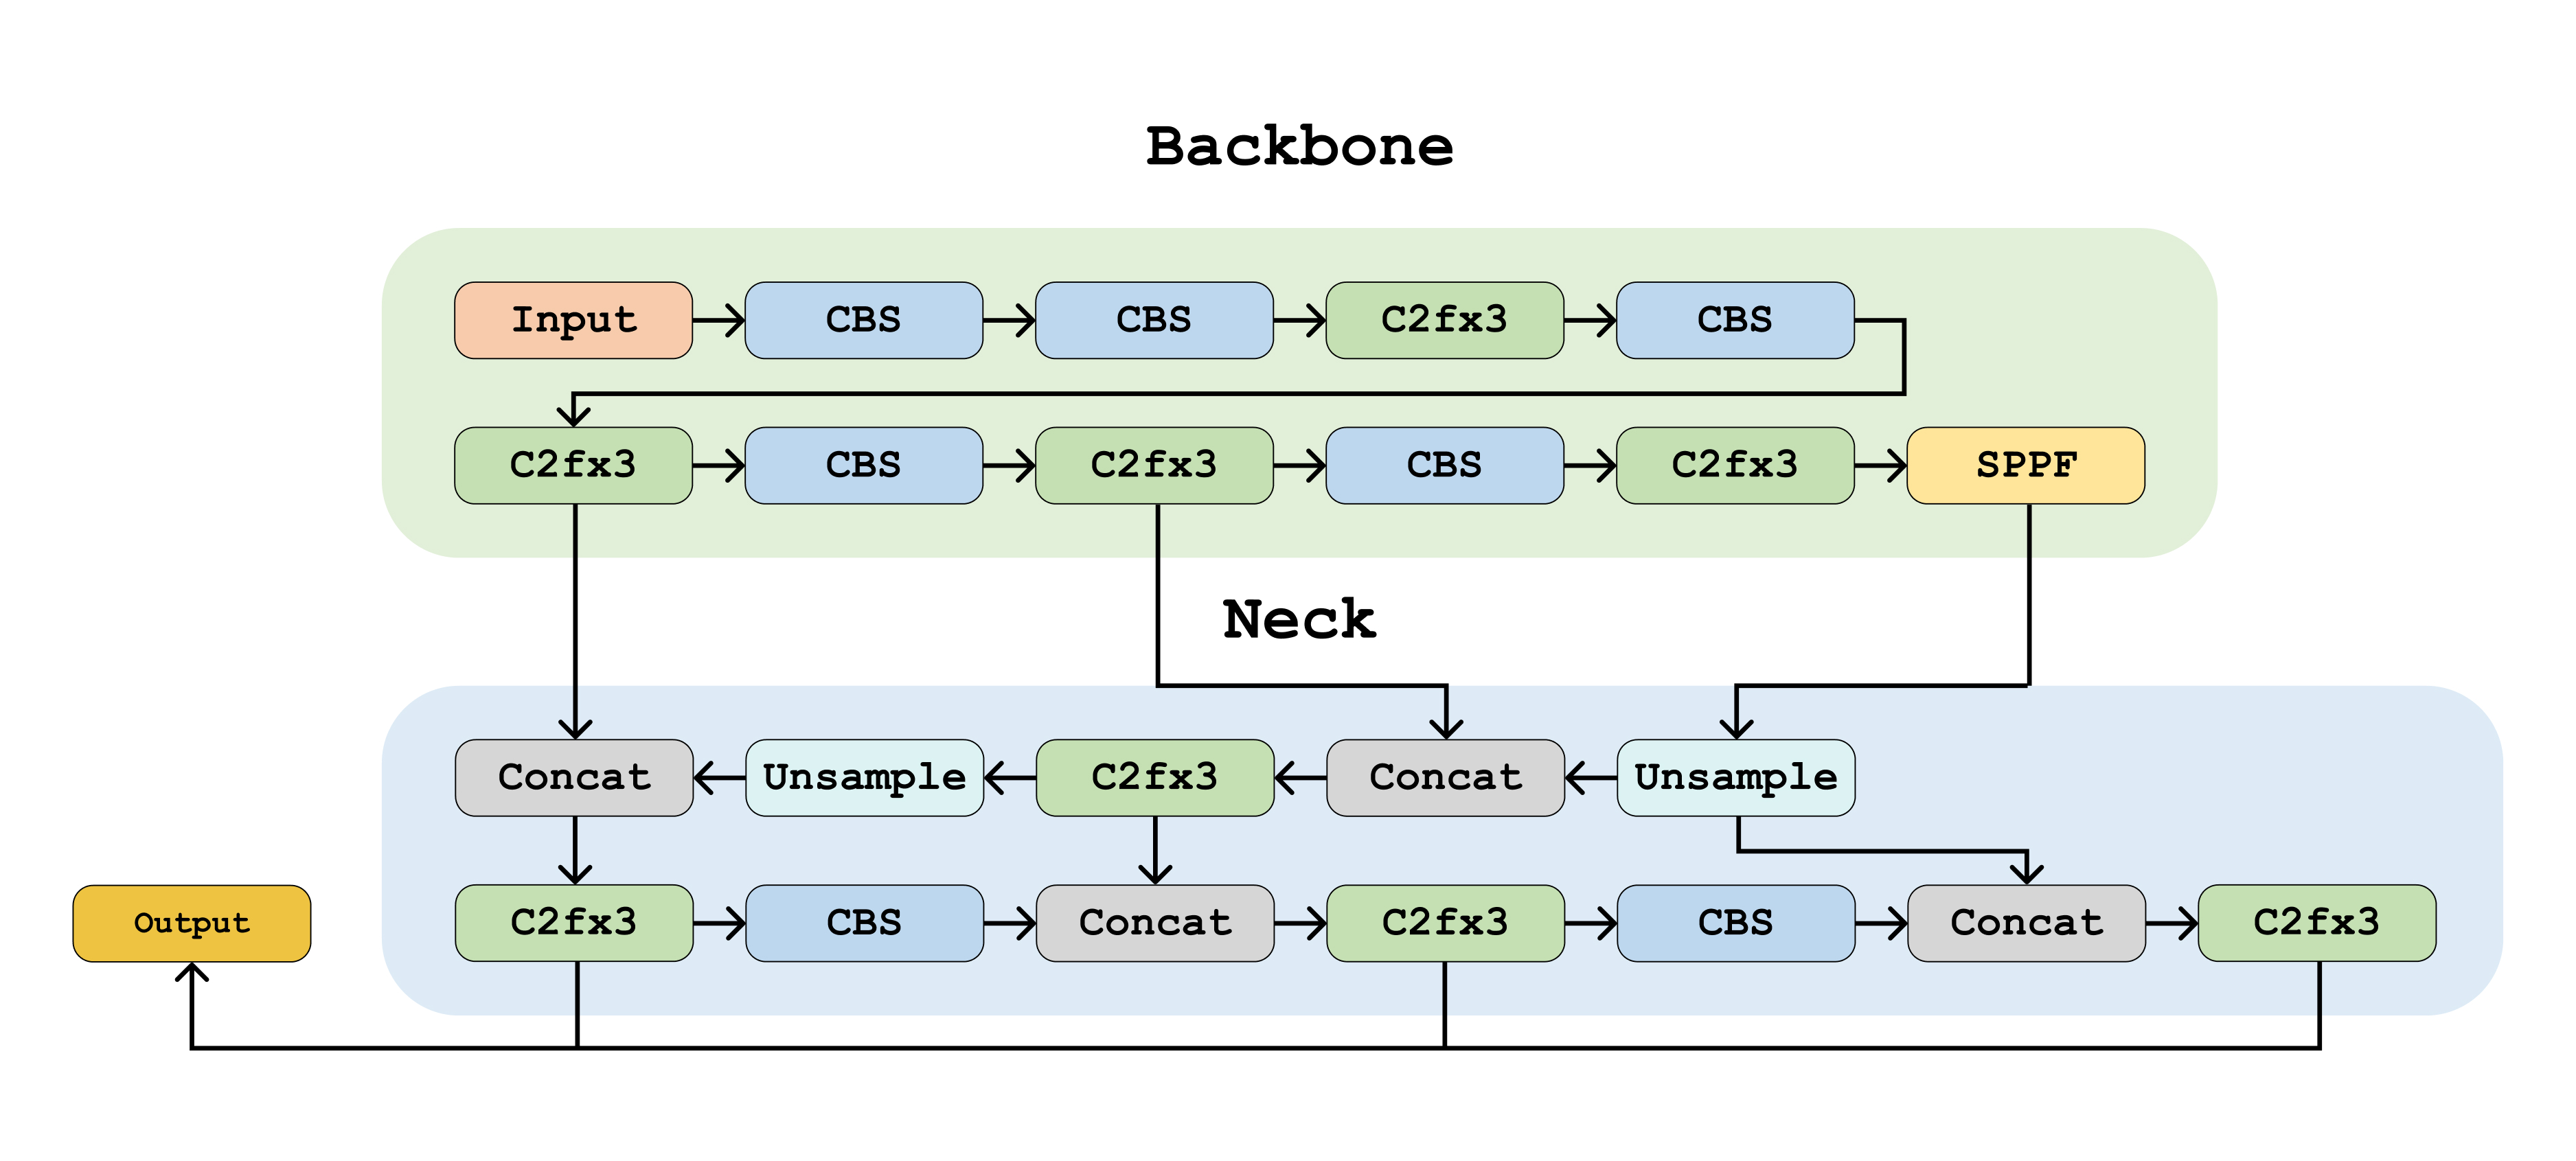
\includegraphics[width=0.85\textwidth]{6-1}
    \caption{Схема структуры модели YOLOv8}
    \label{img:6-1}
\end{figure}

Одними из главных нововведений YOLOv8, представляющими интерес в данной работе, являются встроенные алгоритмы трекинга -- BoT-SORT \cite{6-8} и ByteTrack \cite{6-9}. 

\subsection{StrongSORT}

StrongSORT -- алгоритм трекинга, являющийся улучшением алгоритма DeepSORT, который, получая на вход данные с этапа детектирования, использует дескриптор описания объектов для получения особенностей изображений объектов и  построения коэффициента сходства между траекторией и новым срабатыванием детектора, повышая качество отслеживания объектов.

\vspace{0.3cm}

\begin{figure}[ht]
    \centering
    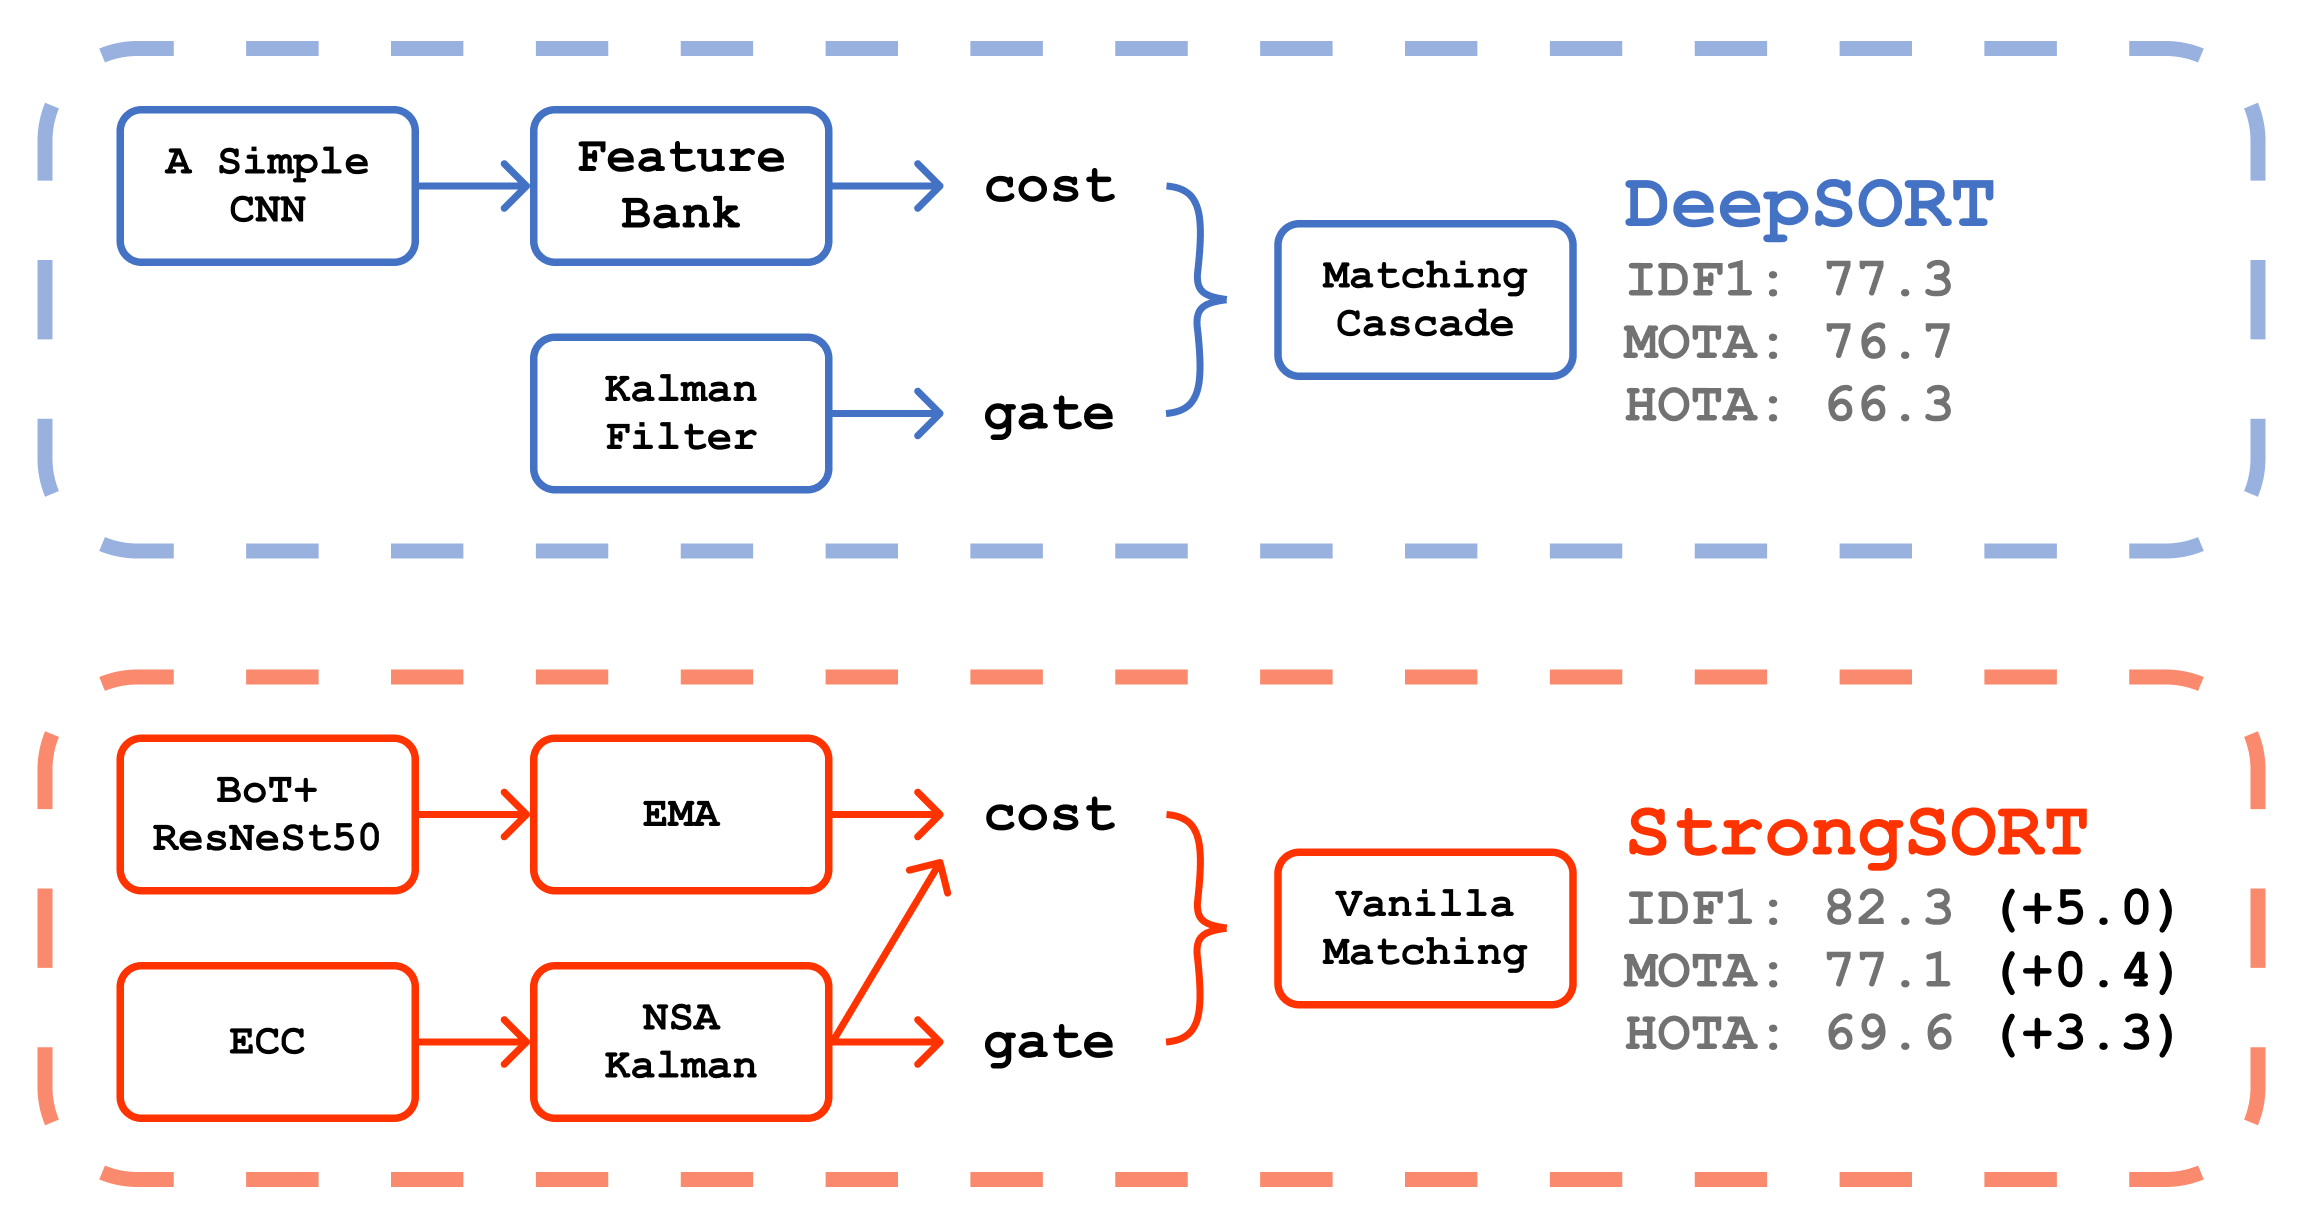
\includegraphics[width=0.85\textwidth]{7-1}
    \caption{Сравнение DeepSORT и StrongSORT}
    \label{img:7-1}
\end{figure}

\textbf{Улучшенные модули.} Faster R-CNN и CNN из DeepSORT заменены на YOLOX-X \cite{7-1} и BoT \cite{7-2}, позволяющие извлекать большее количество признаков объектов.

\vspace{0.2cm}

\textbf{EMA (Exponential Moving Average).} Механизм feature bank, чувствительный к шуму \cite{7-3}, заменяется новой стратегией обновления признаков, использующей межкадровую информацию и снижающей уровень шума при обнаружении, что не только улучшает качество сопоставления, но и сокращает временные затраты \cite{7-4}.

\vspace{0.2cm}

\textbf{ECC (Enhanced Correlation Coefficient).} Для уменьшения влияния движения камеры вводится метод параметрического выравнивания изображений, оценивающий глобальное изменение движения камеры между кадрами \cite{7-5}. Его основу представляет следующий критерий для количественной оценки работы межкадрового преобразования:

    \begin{equation}
        E_{ECC}(p) = \norm{ \frac{\bar{i}_r}{\norm{\bar{i}_r}} - \frac{\bar{i}_w(p)}{\norm{\bar{i}_w(p)}} }^2,
    \end{equation}

\noindent где $\norm{\cdot}$ -- евклидова норма, $p$ -- параметр преобразования, $\bar{i}_r$ и $\bar{i}_w(p)$ -- изначальное и преобразованное изображения с нулевым средним. Далее задача выравнивания решается путем минимизации $E_{ECC}(p)$ с предложенным прямым аддитивным итерационным алгоритмом или обратным композиционным итерационным алгоритмом.

\vspace{0.2cm}

\textbf{NSA Kalman.} Классическая версия фильтра Калмана чувствительна к обнаружениям плохого качества и игнорирует информацию о масштабах шума обнаружения \cite{7-6}. Решением этой проблемы служит NSA Калман из GIAOTracker, предлагающий формулу для адаптивного вычисления шума ковариации $\bar{R_k}=(1-c_k)R_k$, где $R_k$ -- константа шума ковариации по умолчанию, а $c_k$ -- оценка достоверности на шаге $k$. Очевидно, что более высокая оценка $c_k$ соответствует более низкому уровню шума, что и сказывается на низком $\bar{R_k}$.

\vspace{0.2cm}

\textbf{Motion Cost.} Используется как информация о внешнем облике объекта, так и информация о его передвижении.

\vspace{0.2cm}

\textbf{Vanilla Matching.} Каскадный алгоритм \cite{7-7} ограничивает производительность трекера, делая его чувствительным к запутанным ассоциациям. В качестве решения данной проблемы он заменяется на алгоритм Vanilla Global Linear Assignment.

\vspace{0.2cm}

\textbf{AFLink.} Для достижения ассоциаций высокой точности во множестве работ часто используется глобальная связь для треклетов. Однако они требуют больших вычислительных затрат и имеют множество гиперпараметров для точной настройки. Например, алгоритм связей в GIAOTracker использует улучшенный ResNet50-TP для извлечения 3D признаков треклетов и выполнения ассоциации с дополнительными пространственными и временными расстояниями. Ему необходимо установить 6 гиперпараметров, что влечет за собой продолжительные эксперименты по настройке и низкую устойчивость. Исходя из этого, предлагается модель, не использующая информацию о внешнем виде, предсказывающая связь объектов между треклетами, полагаясь только на пространственно-временную информацию.

\subsection{GSI}

Для заполнения пропущенных кадров в траектории часто используется метод интерполяции, востребованный благодаря простоте реализации. Однако его точность ограничена отсутствием использования информации о движении, играющем огромную роль в видео с беспилотных летательных аппаратов. В связи с этим рассматривается интерполяционная модель GSI, использующая регрессию на основе гауссовского процесса \cite{8-1}.

Для $i$-ой траектории модель строится следующим образом:
\begin{equation*}
    p_t = f^{(i)}(t)+\epsilon,
\end{equation*}
где $t \in F$ -- номер кадра, $p_t \in P$ -- координаты положений в кадре $(x, y, w, h)$ и $\epsilon \sim N(0, \sigma^2)$ -- гауссовский шум.

Располагая полученными после трекинга и интерполяции траекториями $S^{(i)}={t^{(i)}, p^{(i)}_t}^L_{t=1}$ длины L, задача моделирования нелинейного движения решается путем определения функции $f^{(i)}$. Предполагается, что она описывается гауссовским процессом:

\begin{equation}
    f^{(i)} \in GP(0, k(\cdot, \cdot)),
\end{equation}

\noindent где $k(x, x')=exp(- \frac{||x-x'||^2}{2 \lambda^2})$ -- ядро радиальной базисной функции.

В результате получения множества кадров $F^*$, согласно свойствам гауссовских процессов, сглаженные координаты $P^*$ определяются следующим образом:

\begin{equation}
    P^*=K(F^*,F)(K(F,F) + \sigma^2 I)^{-1}P,
\end{equation}

\noindent где $K(\cdot, \cdot)$ -- функция ковариации для $k(\cdot, \cdot)$.

Наряду с этим существует гиперпараметр $\lambda$, отвечающий за степень гладкости траектории, связанный с ее длиной. Из данных соображений определена следующая функция:

\begin{equation}
    \lambda = \tau \cdot \log{\tau^3 / l},
\end{equation}

\noindent где $\tau$ задается по умолчанию равным 10 по результатам экспериментов.

На Рис. \ref{img:8-1} представлено сравнение GSI, линейной интерполяции и необработанной траектории. Полученные в результате трекинга данные обычно содержат в себе неустойчивый характер шума, тогда как линейная интерполяция игнорирует информацию о движении. Для устранения данных помех модель GSI применяет сглаживание всей траектории при участии контролирующего параметра.

\begin{figure}[ht]
    \centering
    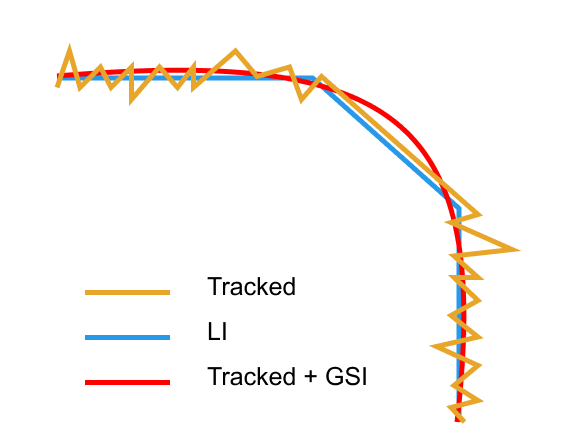
\includegraphics[width=0.85\textwidth]{8-1}
    \caption{Сравнение необработанной траектории (Tracked),\\ линейной интерполяции (LI)\\ и интерполяции с гауссовским сглаживанием (Tracked + GSI)}
    \label{img:8-1}
\end{figure}

\section{Основная часть}

Основная часть данной работы состоит из подготовки данных, обучения модели детектирования объектов, применения алгоритма трекинга, проведения постобработки и анализа полученных результатов.

\subsection{Подготовка данных}

В задаче классификации нередко возникают ситуации, когда в обучающей выборке доли объектов различных классов существенно разнятся, создавая так называемую проблему несбалансированности классов \cite{9-1}, негативно влияющую на результат работы моделей.

У используемого в данной работе датасета VisDrone существует две особенности, вызывающие проблемы с детектированием: несбалансированность классов и малое количество аннотаций для сценариев плотного расположения групп объектов малого размера.

Для решения первой проблемы были использованы аугментации для искусственного увеличения количества изображений с объектами малопредставленных классов, идея чего вдохновлена методом перебалансировки данных Synthetic Minority Over-Sampling Technique (SMOTE) \cite{9-2}, предполагающем увеличение объема миноритарных классов в дополнение к уменьшению объема мажоритарных классов. Так как при классическом использовании удаления объектов преобладающих классов возможно удаление ключевых сценариев \cite{9-3}, в работе использовано только искусственное увеличение количества объектов малопредставленных классов.

Был проведен анализ датасета с целью выявления для каждого класса видеопоследовательностей с наибольшим количеством объектов из него. Для каждой такой видеопоследовательности были найдены кадры с наиболее плотным скоплением объектов из соответствующего класса, как показано на Рис. \ref{img:9-1}. Далее по координатам из аннотаций найденные области были вырезаны и увеличены, после чего к ним были применены операции аугментации во избежание переобучения модели на одинаковых кадрах, а именно различные повороты, позволившие значительно увеличить количество объектов в малопредставленных классах, как на Рис. \ref{img:9-2} и \ref{img:9-3}.

\vspace{0.5cm}

\begin{figure}[ht]
    \centering
    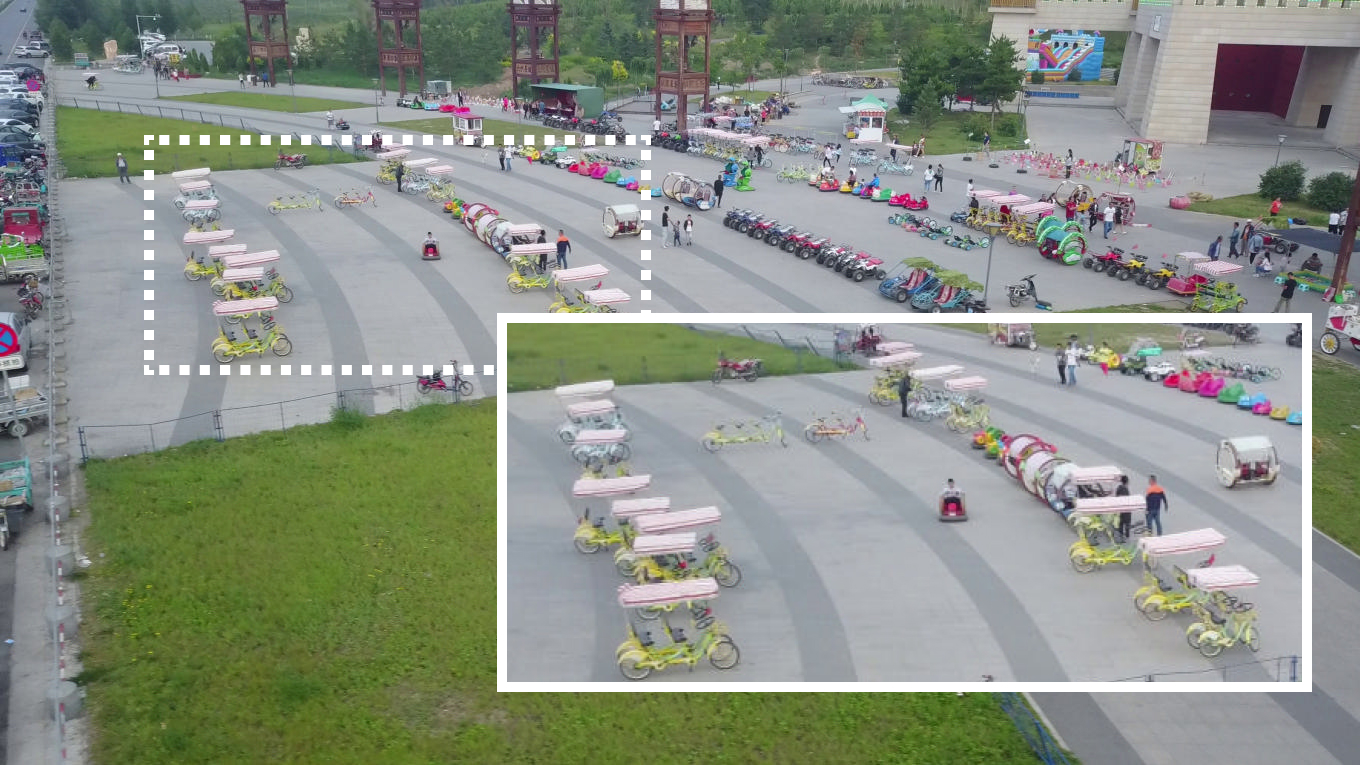
\includegraphics[width=0.85\textwidth]{9-1}
    \caption{Пример области с объектами малопредставленного класса}
    \label{img:9-1}
\end{figure}

\begin{figure}[ht]
    \centering
    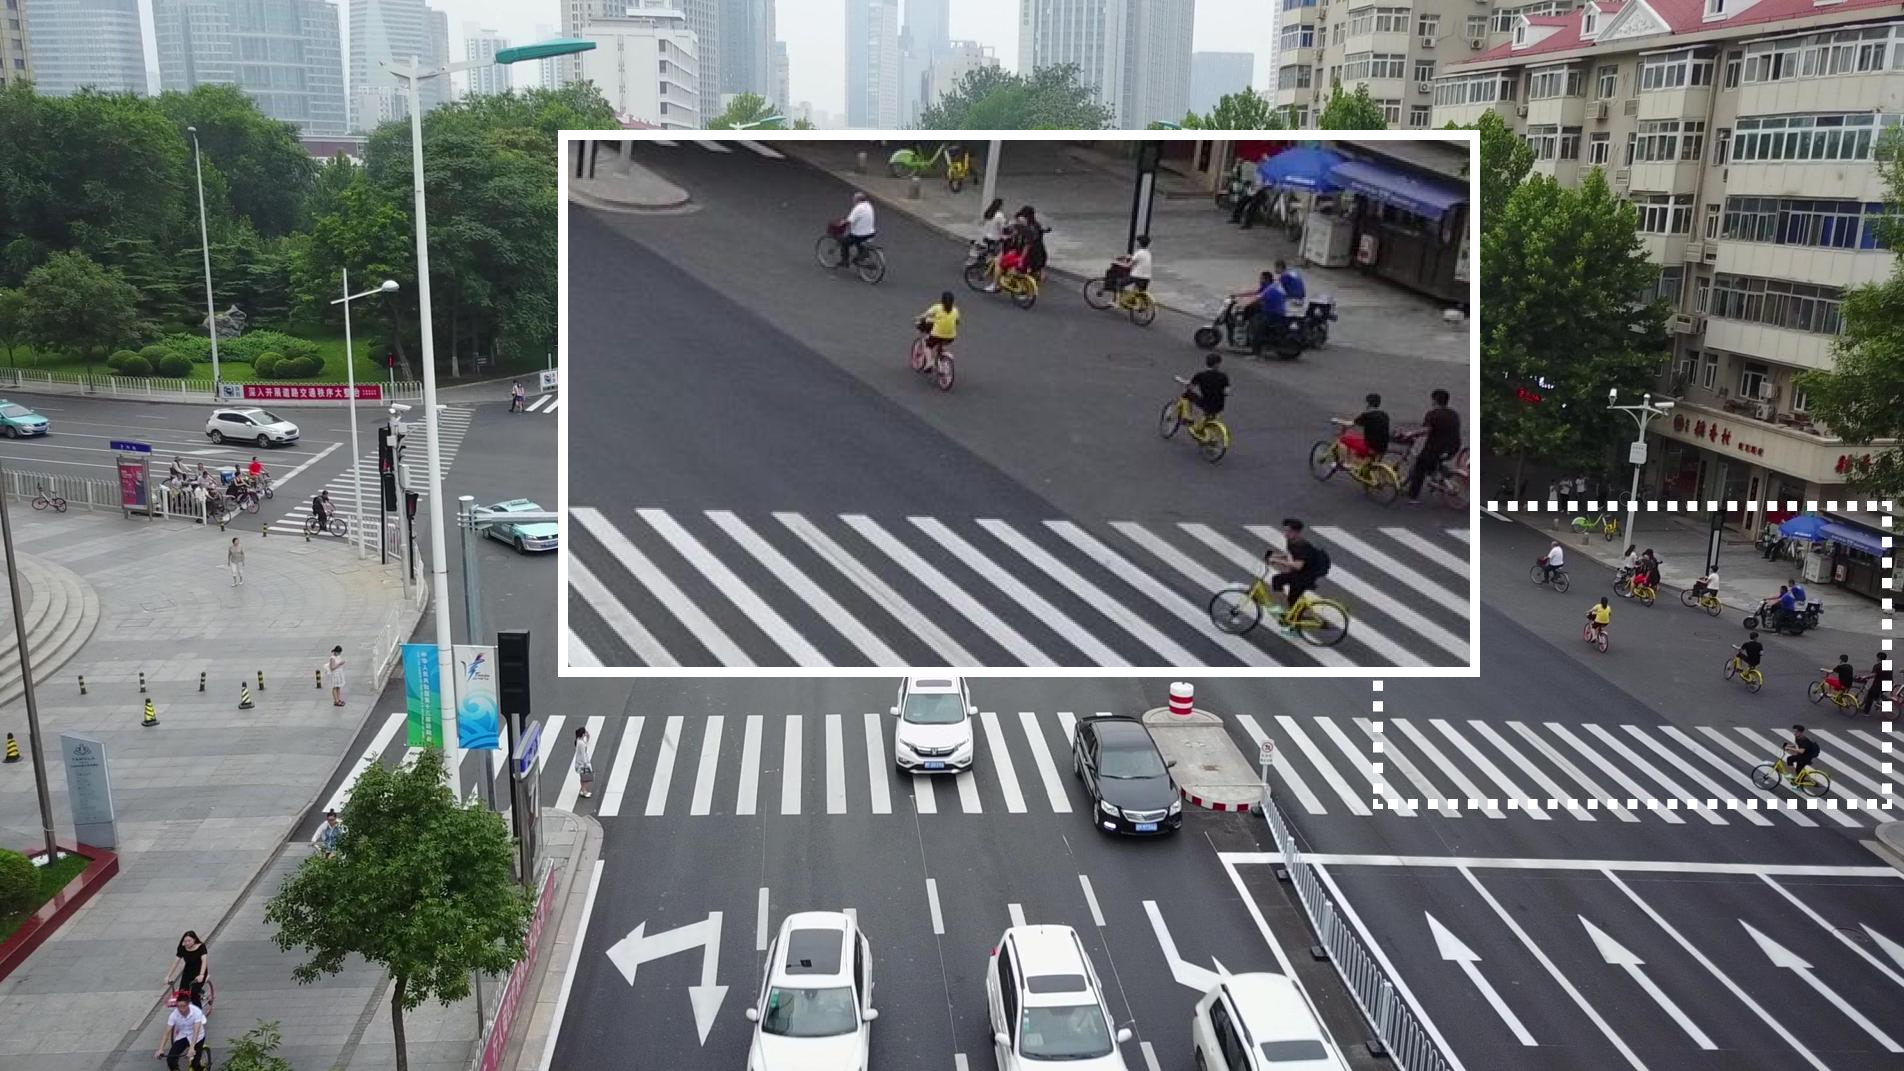
\includegraphics[width=0.85\textwidth]{9-2}
    \caption{Найденная область с объектами малопредставленного класса}
    \label{img:9-2}
\end{figure}

\begin{figure}[ht]
    \centering
    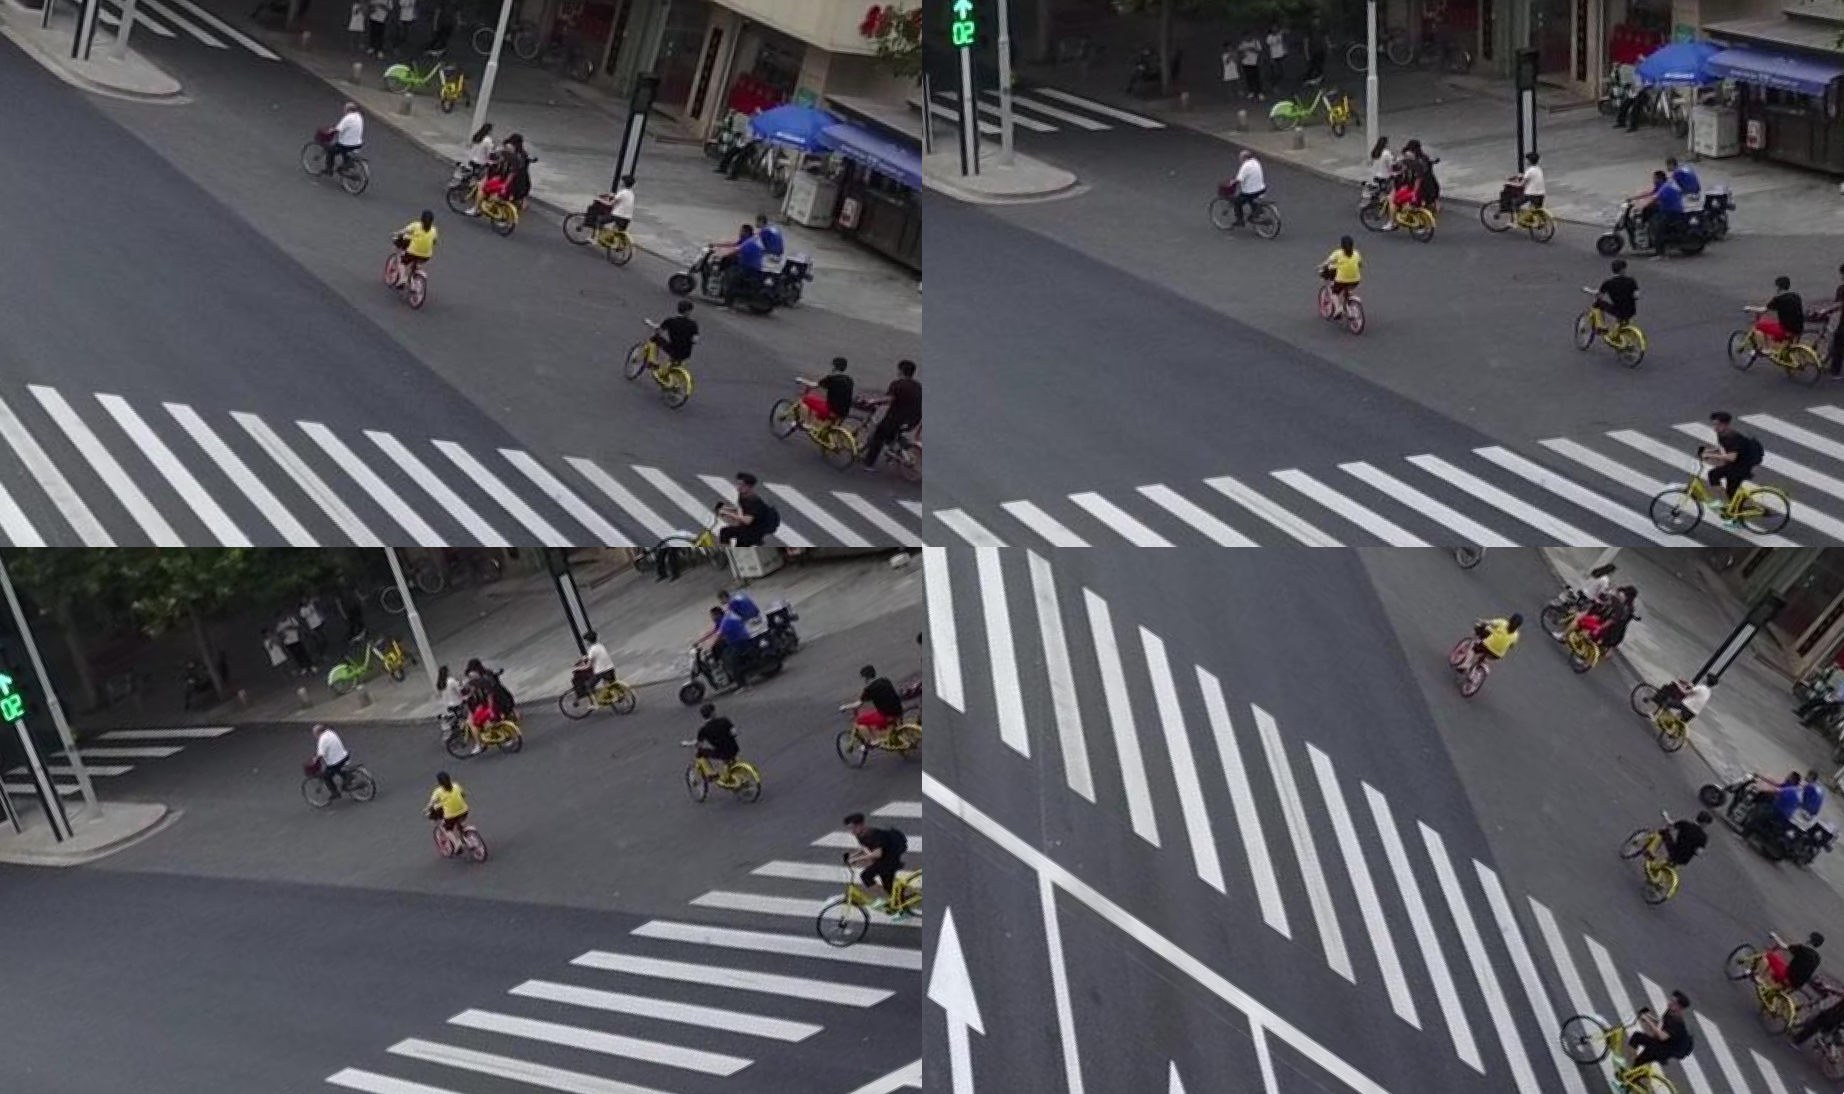
\includegraphics[width=0.85\textwidth]{9-3}
    \caption{Аугментации поворотами полученной области}
    \label{img:9-3}
\end{figure}

Проделанная работа помогла уравновесить количество объектов в классах, несбалансированность которых была представлена на Рис. \ref{img:3-3}, результат чего можно увидеть на Рис. \ref{img:9-4}.

\begin{figure}[ht]
    \centering
    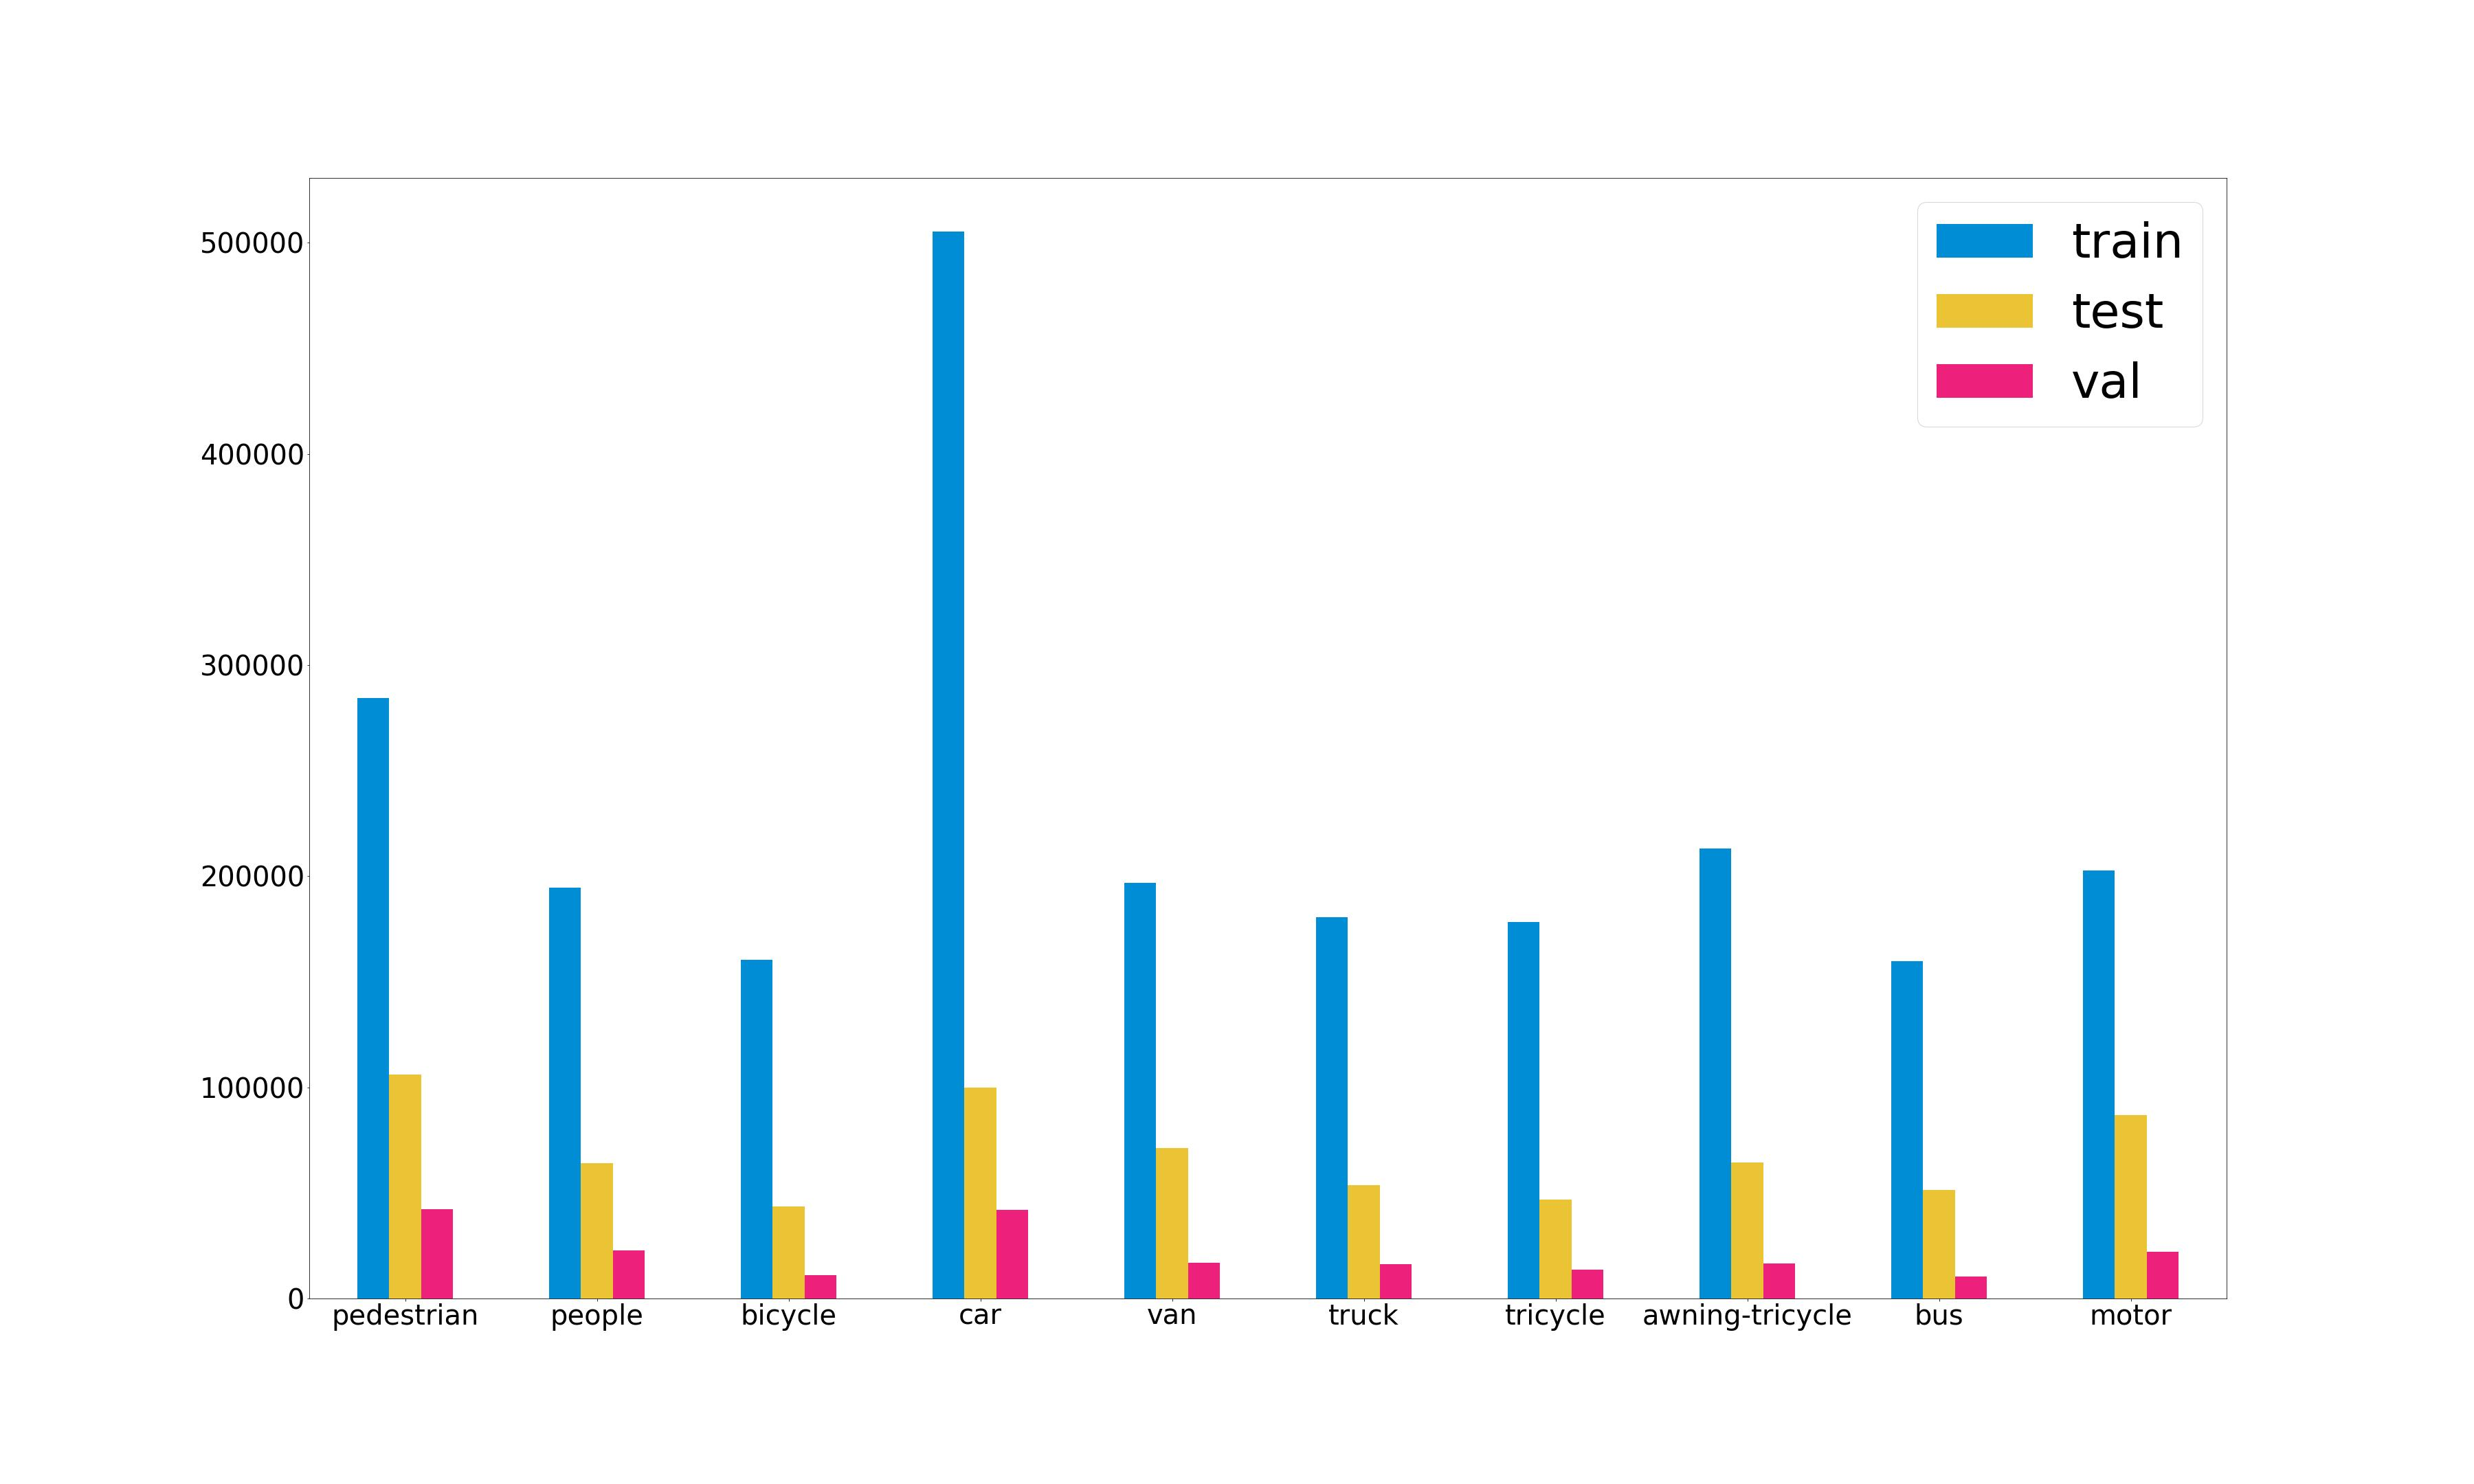
\includegraphics[width=0.85\textwidth]{9-4}
    \caption{Новое распределение объектов по классам}
    \label{img:9-4}
\end{figure}

Для решения второй вышеприведенной проблемы был дополнительно использован датасет UAVDT по причине наличия в нем множества сценариев плотного расположения объектов. После проведения анализа датасета были выбраны видеопоследовательности с наибольшим количеством объектов в кадре, как на Рис. \ref{img:9-5}, большая часть которых отобрана по наличию в атрибутах датасета меток о высокой точке обзора. 

\vspace{0.5cm}

\begin{figure}[ht]
    \centering
    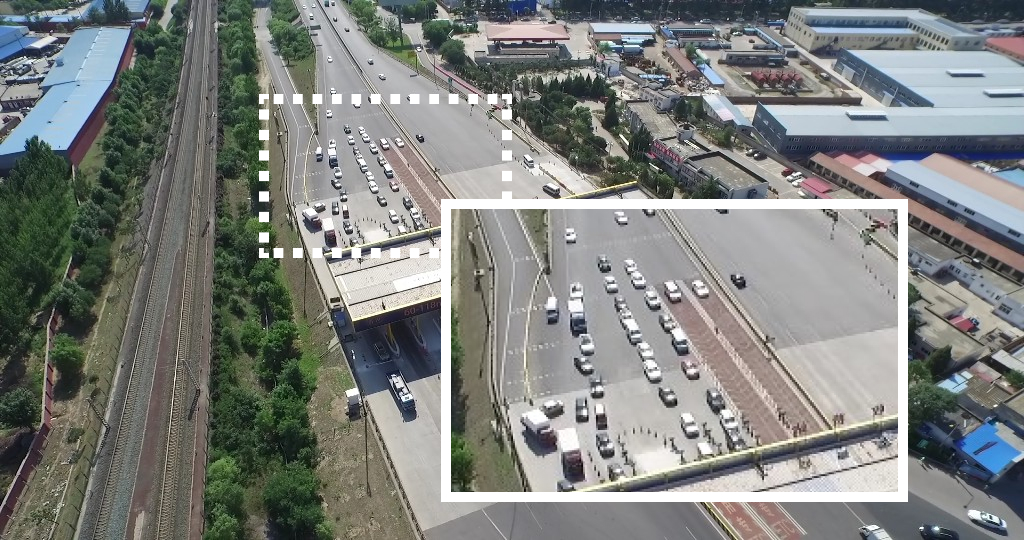
\includegraphics[width=0.85\textwidth]{9-5}
    \caption{Пример области с плотным расположением объектов малого размера}
    \label{img:9-5}
\end{figure}

\subsection{Покадровое детектирование}

В начале работы над этапом детектирования было запущено обучение модели YOLOv5m на датасете VisDrone длительностью в 50 эпох, результатом которого стал $mAP \ 30.0$, в связи с чем был проведен анализ плохо детектируемых объектов, которыми оказались малопредставленные в датасете классы, такие как bus, tricycle и truck, что следует из Рис. \ref{img:10-1} и \ref{img:10-2}, а также объекты малого размера, в частности, в плотных группах на заднем плане.

\vspace{0.5cm}

\begin{figure}[ht]
    \centering
    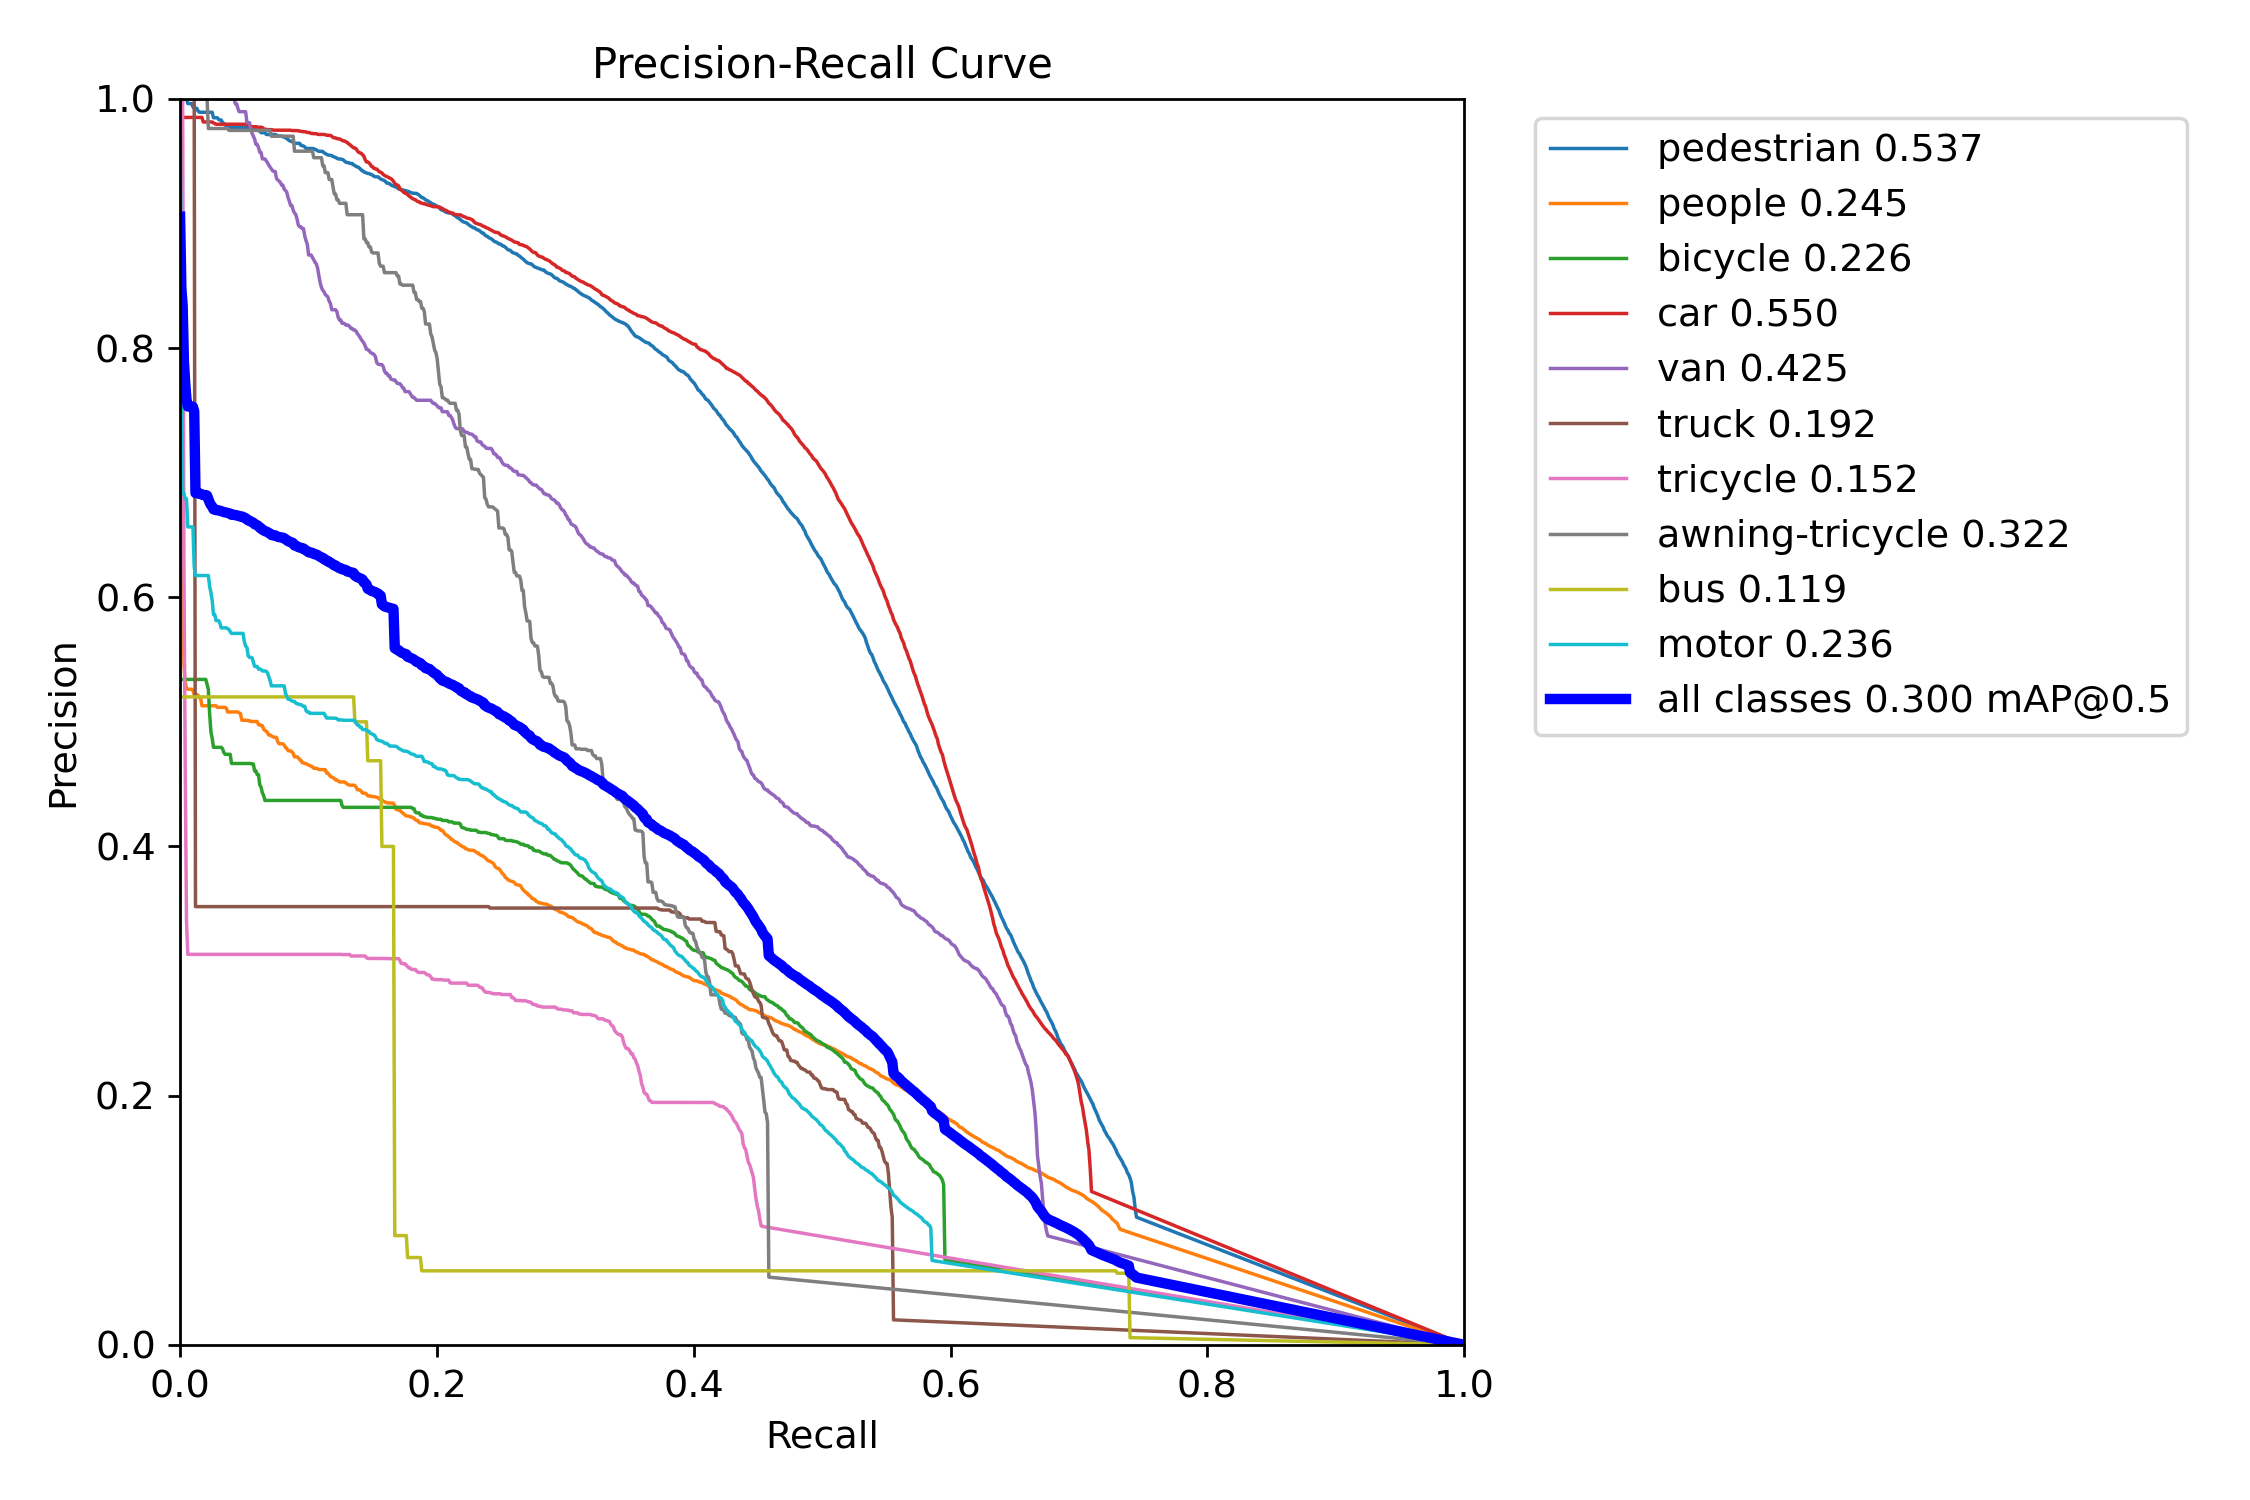
\includegraphics[width=0.85\textwidth]{10-1}
    \caption{Precision-Recall Curve после первого этапа обучения}
    \label{img:10-1}
\end{figure}

\begin{figure}[ht]
    \centering
    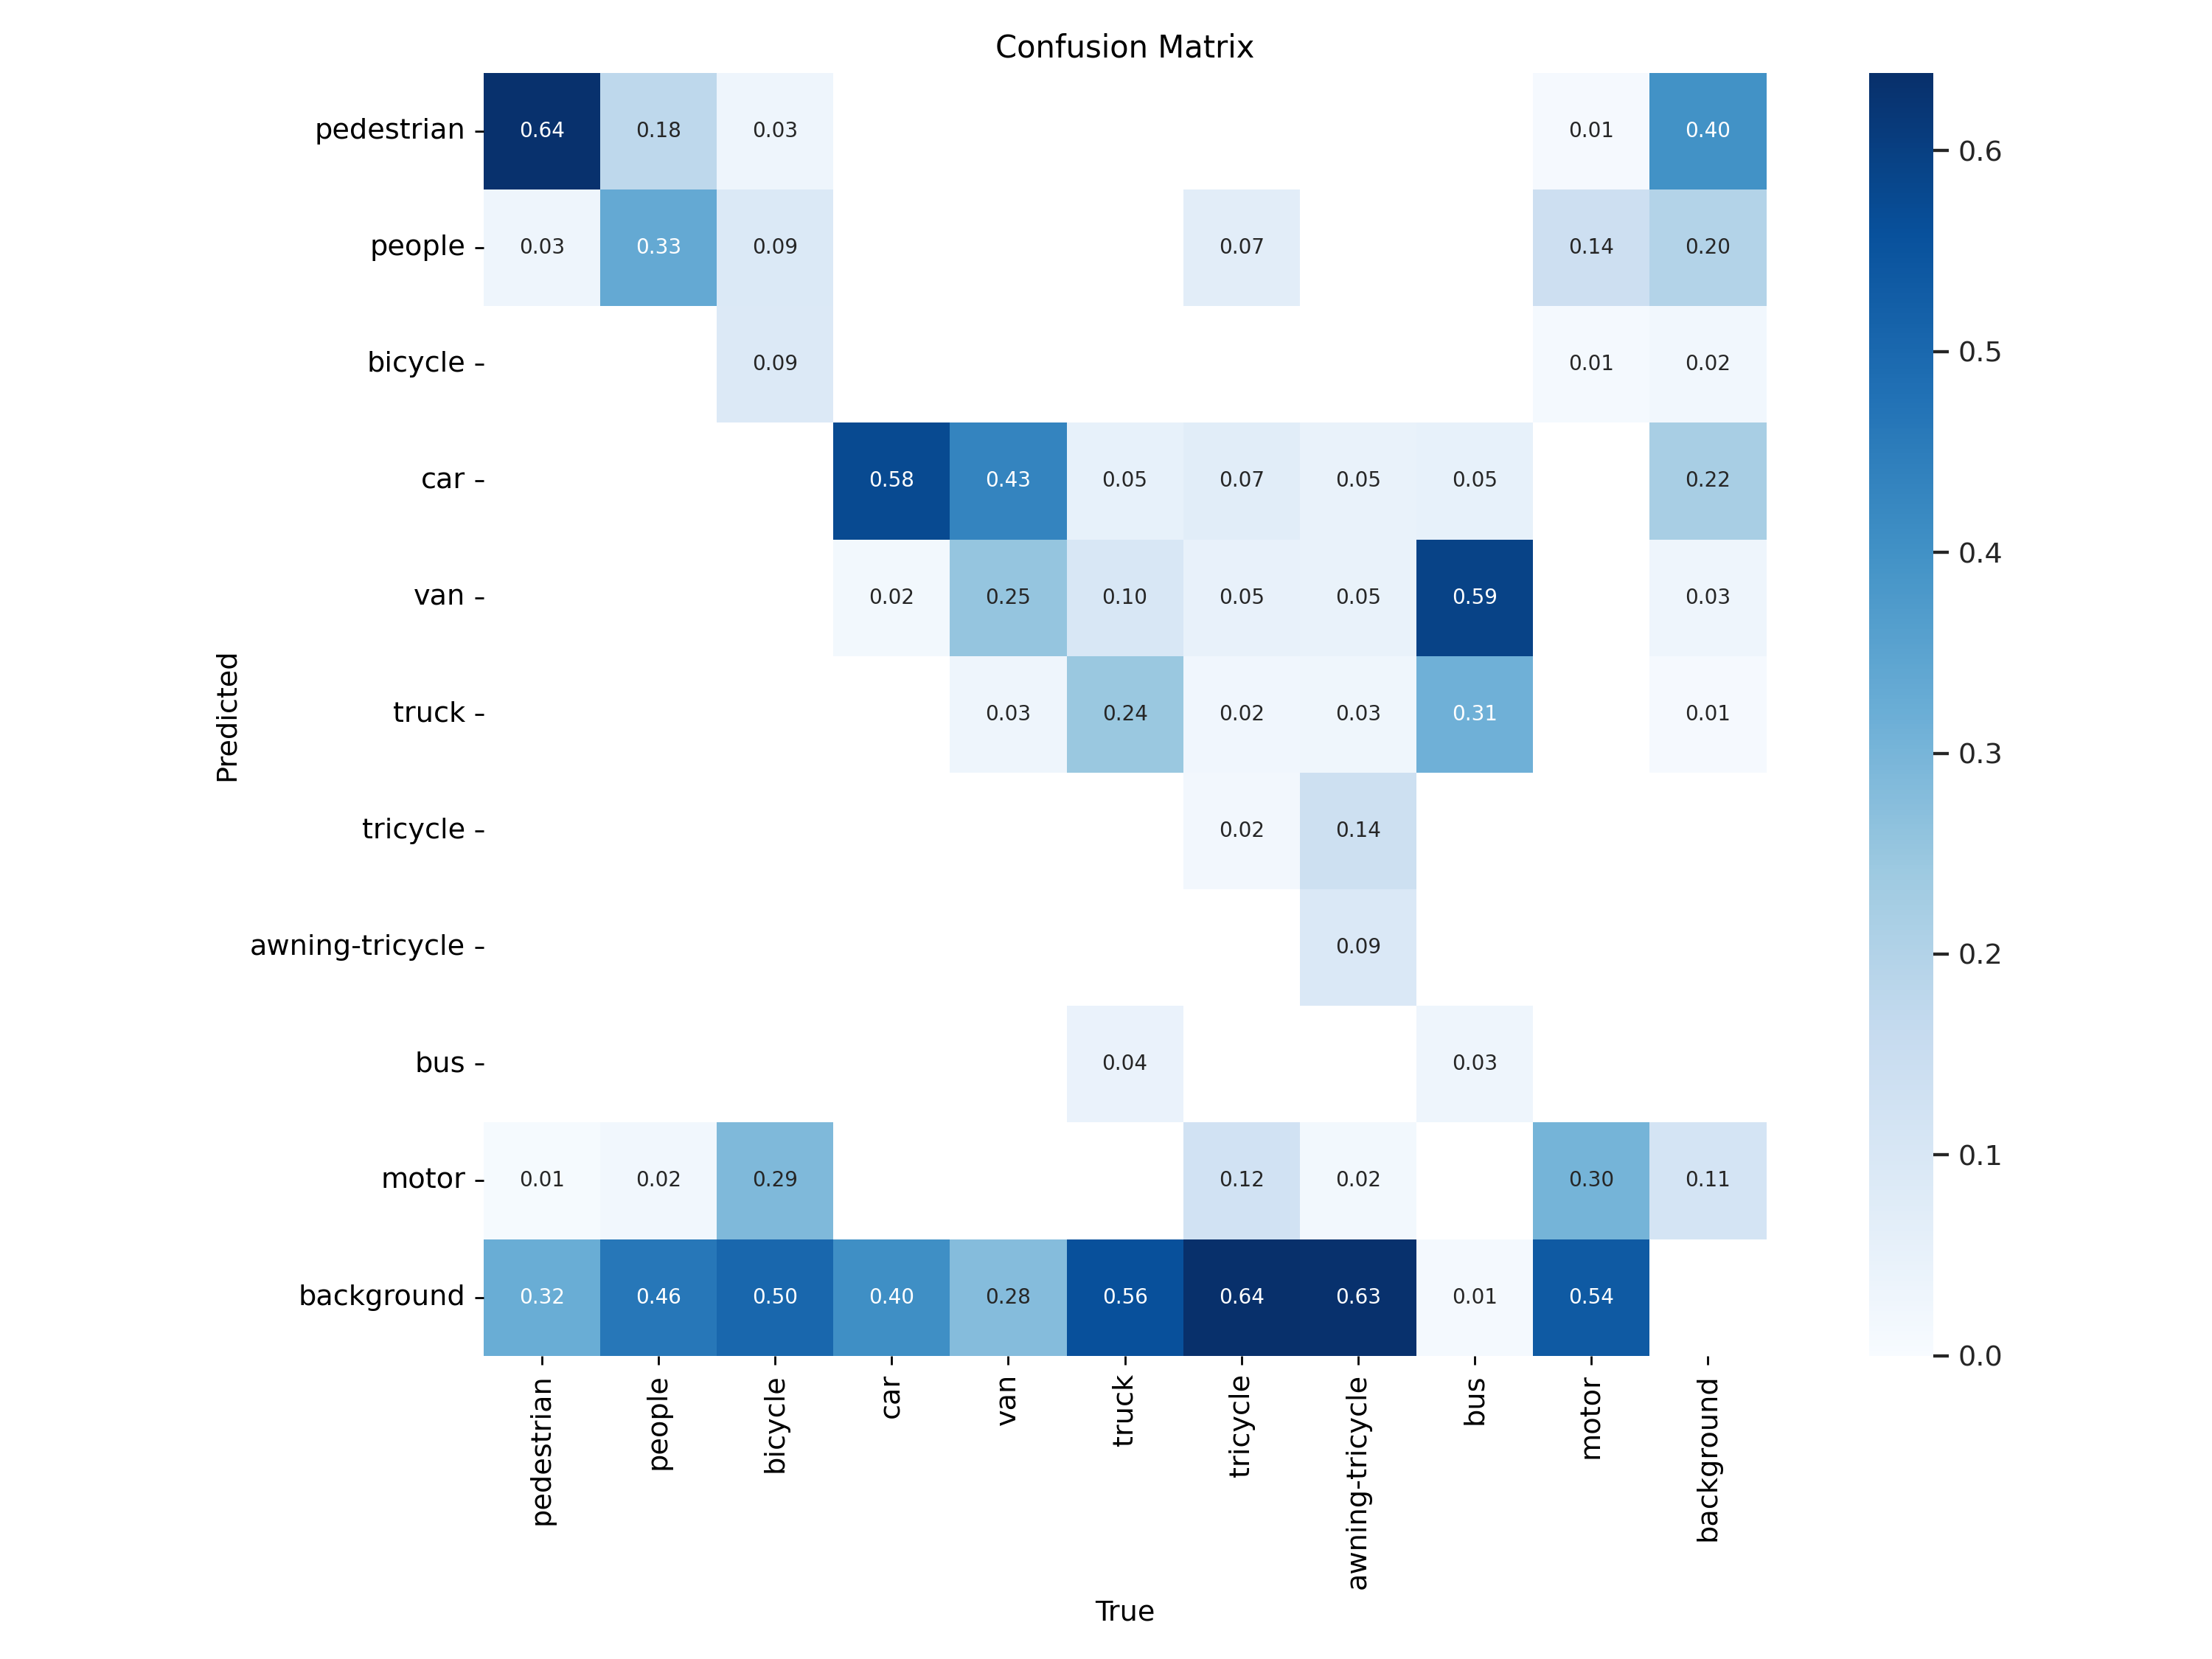
\includegraphics[width=0.85\textwidth]{10-2}
    \caption{Confusion Matrix после первого этапа обучения}
    \label{img:10-2}
\end{figure}

С целью решения первой из вышеприведенных проблем была поставлена задача улучшения датасета, для чего была проведена описанная ранее в работе обработка данных датасета VisDrone, состоящая из аугментации на этапе подготовки данных. После чего было проведено дополнительное обучение длительностью в 100 эпох более крупной модели YOLOv5x, в результате которого $mAP$ повысился до $45.6$, благодаря более высоким результатам на ранее малопредставленных классах, что видно на Рис. \ref{img:10-3}.

\begin{figure}[ht]
    \centering
    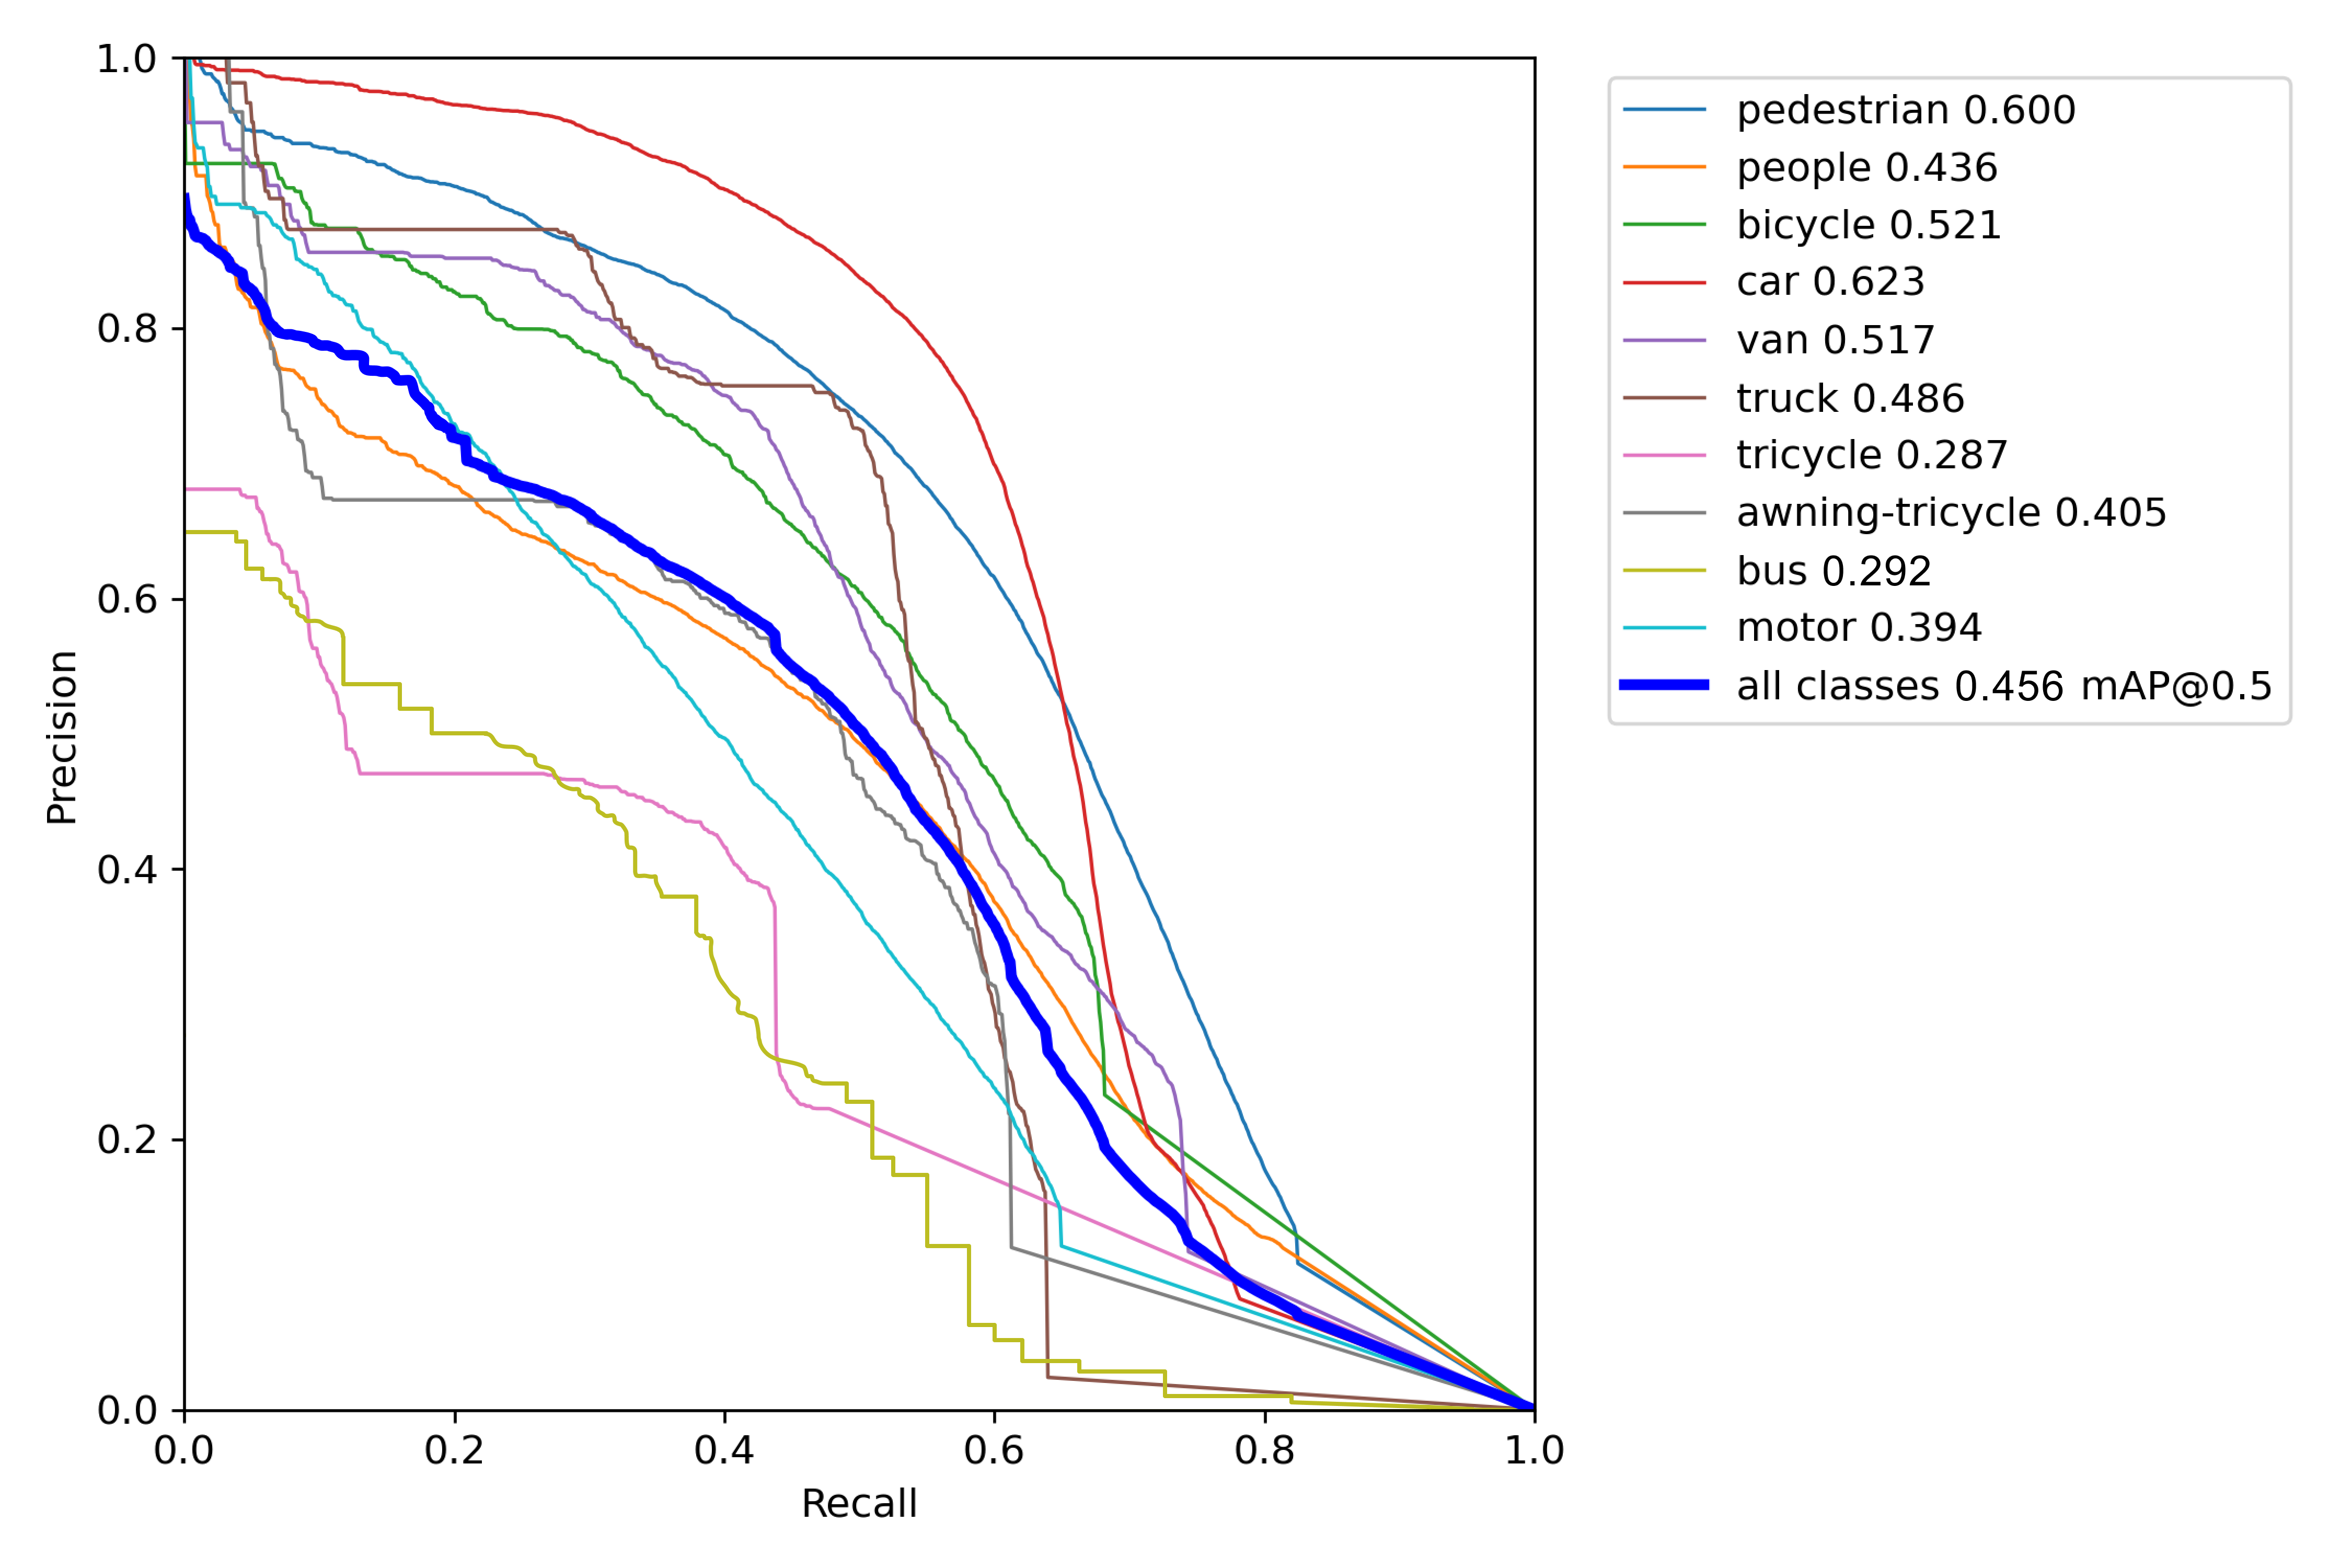
\includegraphics[width=0.85\textwidth]{10-3}
    \caption{Precision-Recall Curve после второго этапа обучения}
    \label{img:10-3}
\end{figure}

Для работы со второй проблемой из вышеуказанных были выполнены подготовка аннотаций для датасета UAVDT, отбор по результатам анализа подходящих видеопоследовательностей из него, содержащих сценарии расположения объектов вдалеке и в плотных скоплениях, а также дообучение длительностью в 50 эпох предыдущей модели, показавшее $mAP \ 48.1$, как на Рис. \ref{img:10-4}.

\vspace{0.5cm}

\begin{figure}[ht]
    \centering
    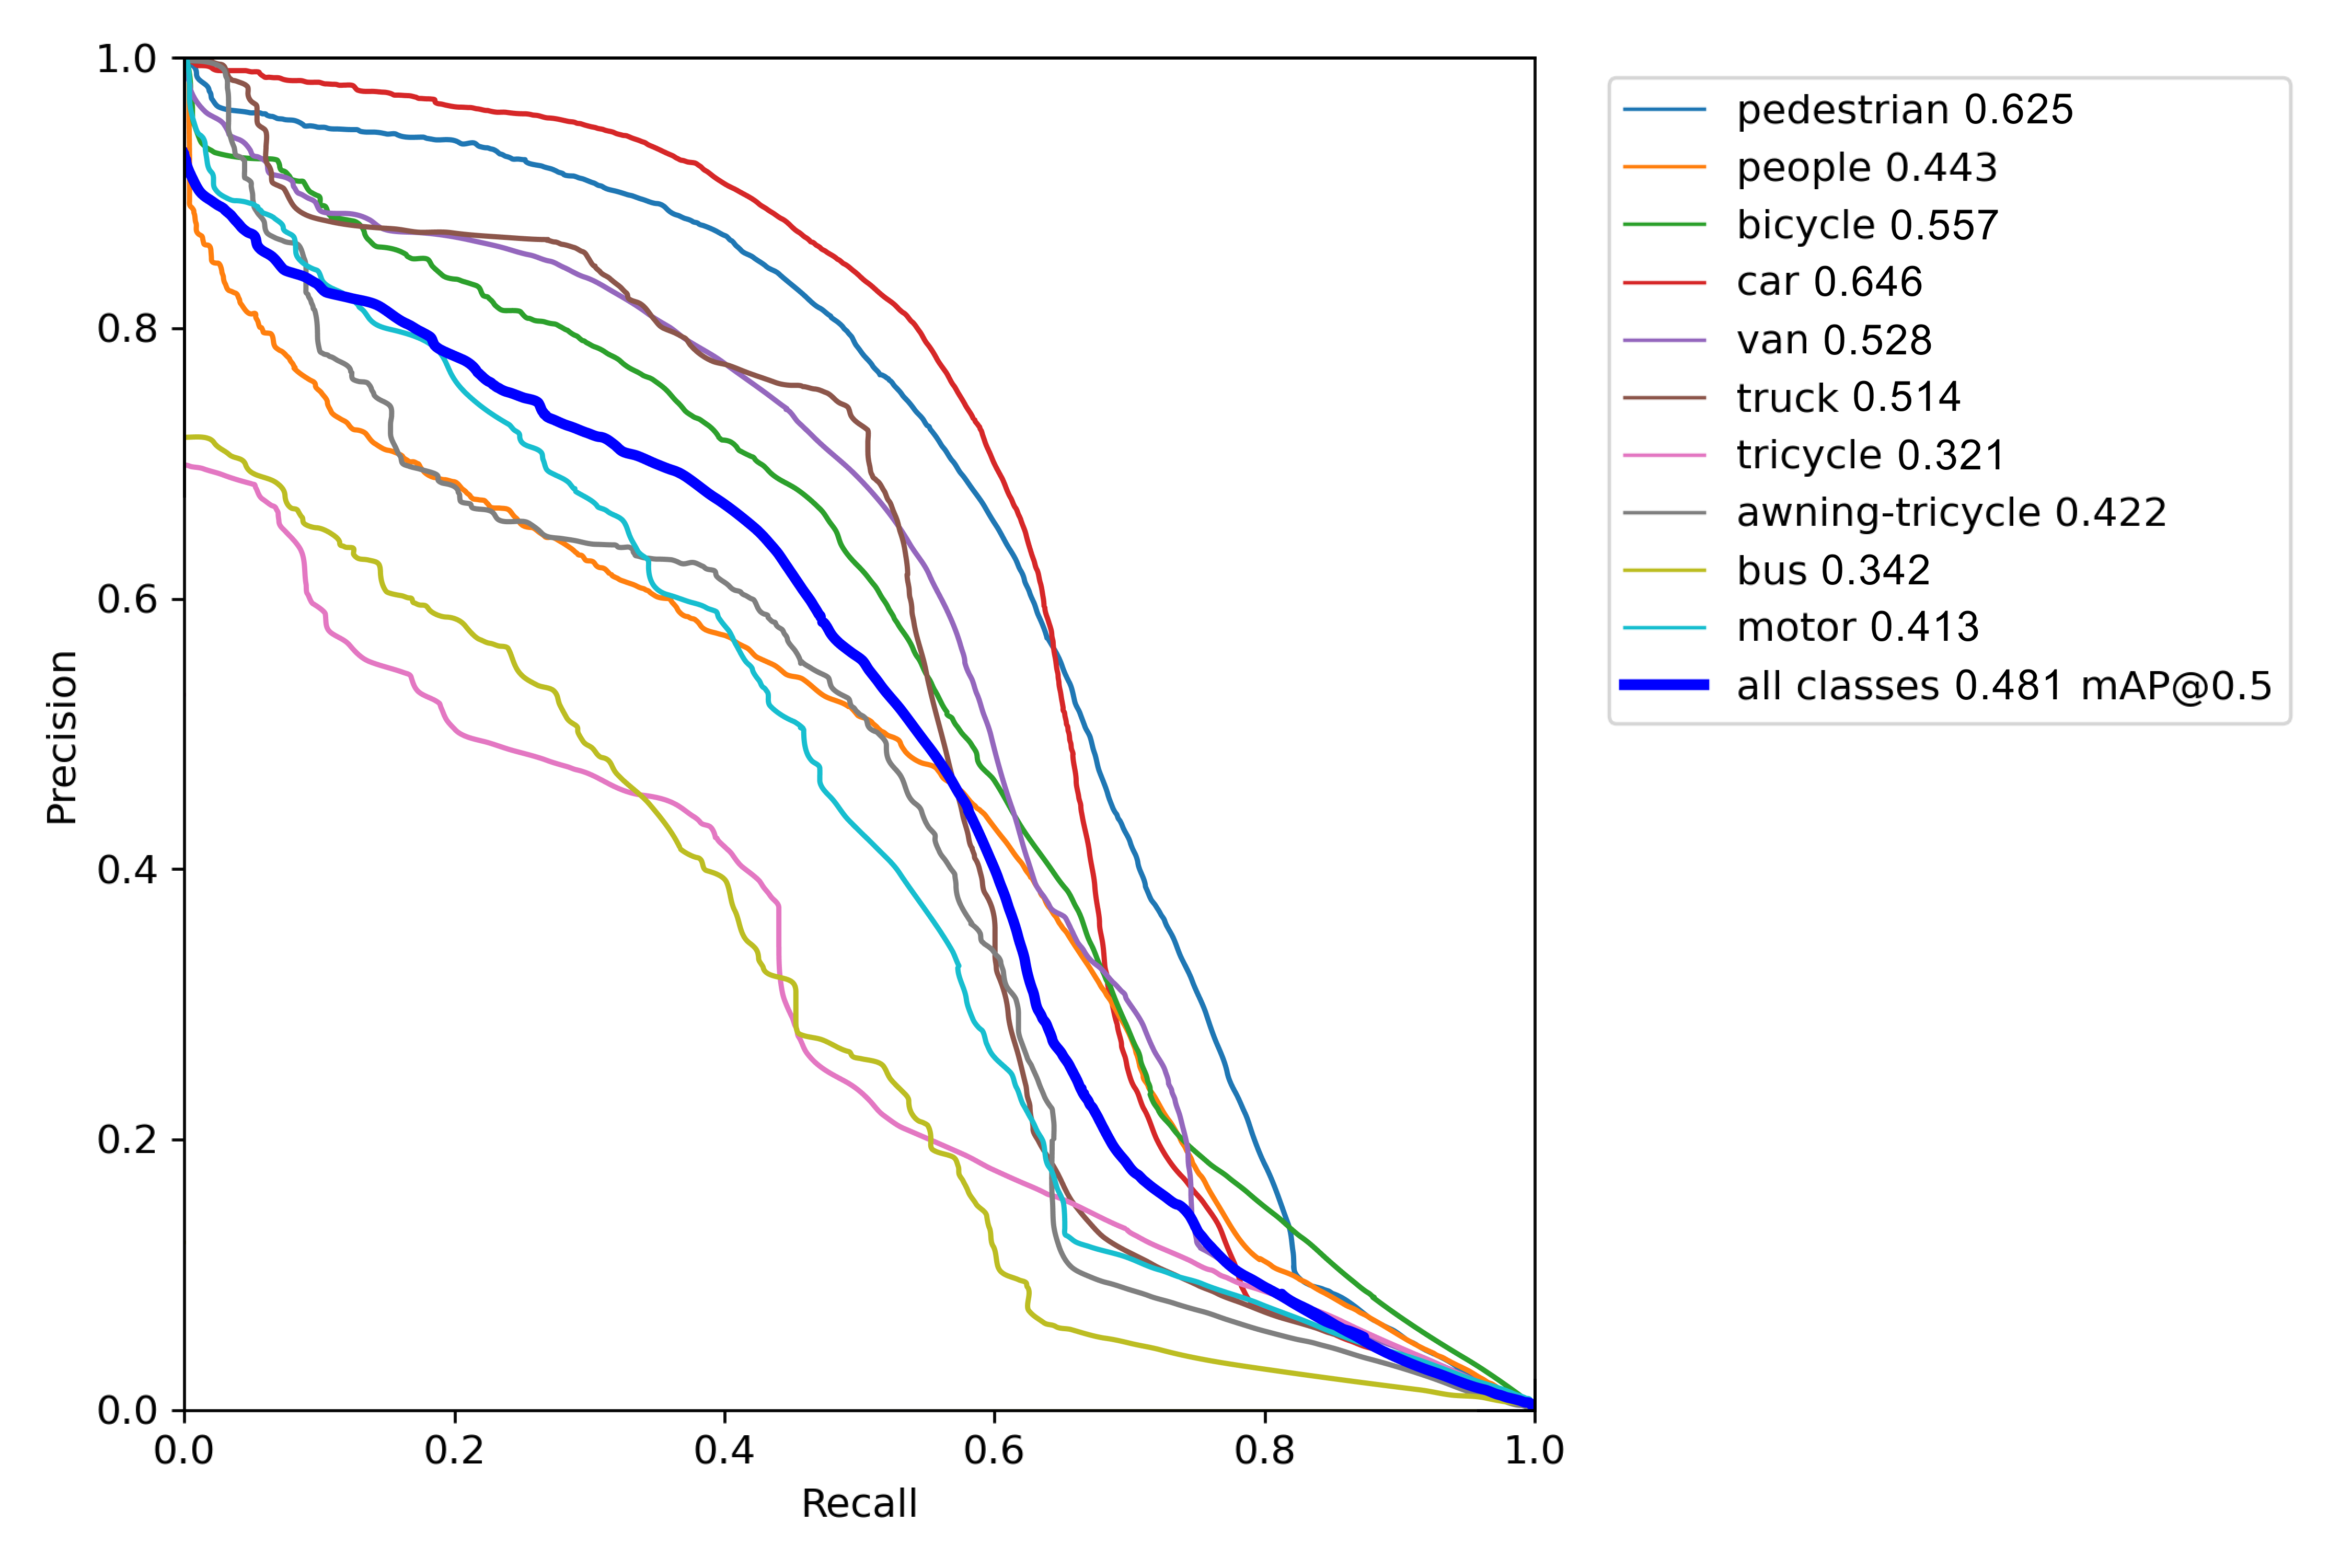
\includegraphics[width=0.85\textwidth]{10-4}
    \caption{Precision-Recall Curve после третьего этапа обучения}
    \label{img:10-4}
\end{figure}

В Таблице \ref{tbl:10-1} представлены результаты обучения на каждом этапе, показавшие значительное улучшение в точности благодаря обработке датасета VisDrone и дообучению на сложных сценариях из датасета UAVDT.

\vspace{0.5cm}

\begin{table}[ht]
    \centering
    \begin{tblr}{c|c}
        \hline[1.5pt]
        Этап & $mAP$ \\
        \hline[1.5pt]
        Без аугментаций & 30.0 \\
        \hline
        Обработка VisDrone & 45.6 \\
        \hline
        Обработка VisDrone + UAVDT & 48.1 \\
        \hline[1.5pt]
    \end{tblr}
    \caption{Результаты на этапе покадрового детектирования}
    \label{tbl:10-1}
\end{table}

\subsection{Трекинг}

После получения результатов модели детектирования было необходимо рассмотреть несколько алгоритмов последующего трекинга, такие как OC-SORT, ByteTrack, DeepSORT и StrongSORT.

Лучшим показавшим себя алгоритмом трекинга для данной задачи по результатам экспериментов стал StrongSORT, который наиболее точно работал с часто пропадающими из кадра и пересекающими траектории друг друга объектами, показав наивысшую из полученных точностей, поскольку одним из главных его преимуществ является способность работать с полными и частичными окклюзиями.

Для данного алгоритма была реализована модификация его официальной версии с целью интеграции с YOLOv5, после чего был проведен запуск трекинга на основе полученной ранее модели детектирования. Пример достигнутого результата приведен на Рис. \ref{img:11-1}, на котором для каждого объекта указаны его класс и уникальный номер.

\vspace{0.5cm}

\begin{figure}[ht]
    \centering
    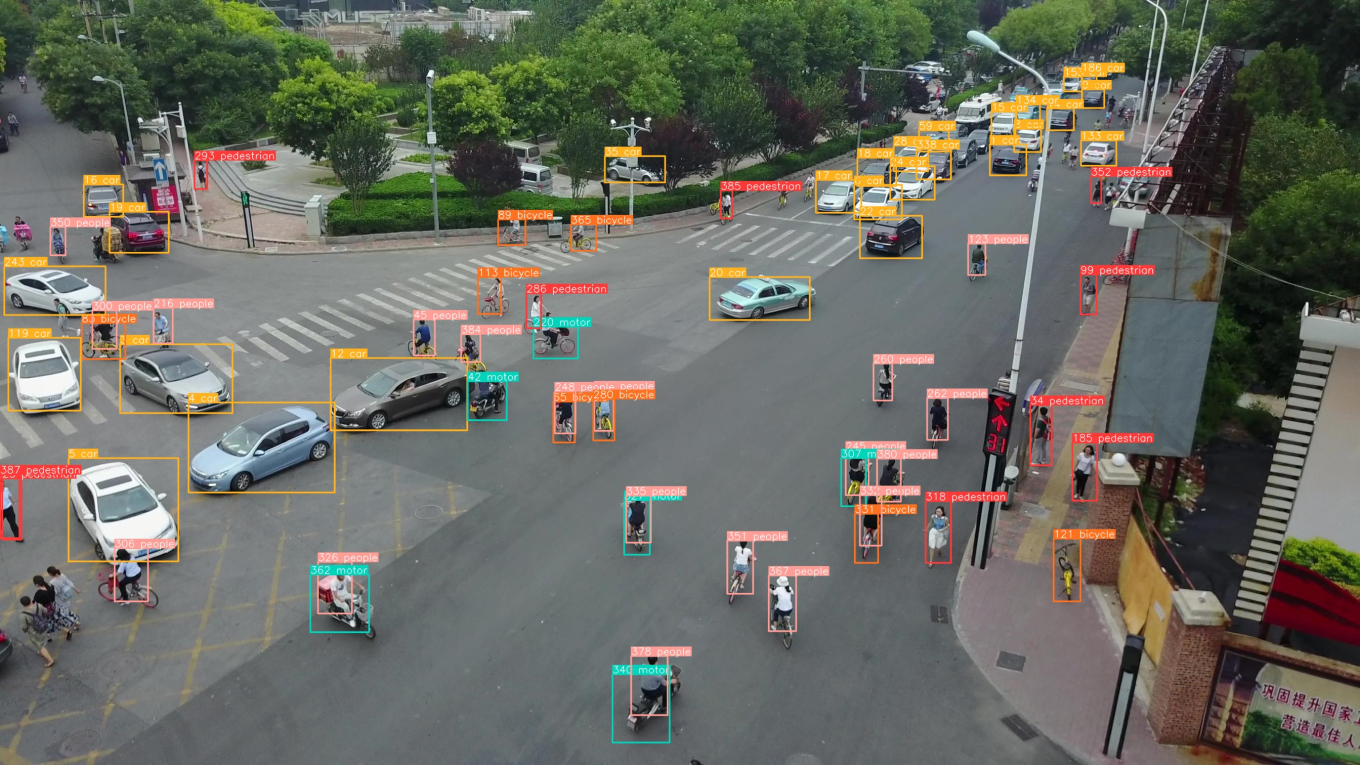
\includegraphics[width=0.85\textwidth]{11-1}
    \caption{Пример кадра из видео, к которому применен алгоритм трекинга StrongSORT}
    \label{img:11-1}
\end{figure}

Однако классический StrongSORT содержит в себе проблемы в построении плавных траекторий объектов по причине наличия нестабильного движения камер с беспилотных летательных аппаратов, вследствие чего некоторые объекты между кадрами теряются, а ограничивающие рамки имеют характер дрожания.

Для решения указанной проблемы в модификацию StrongSORT были добавлены линейная интерполяция и гауссовское сглаживание (GSI), описанные ранее в работе. После применения к трекингу данной постобработки без подбора параметров были получены траектории объектов, нестабильные при резких поворотах и подъемах камер, что наблюдается на Рис. \ref{img:11-2}, где ограничивающие рамки объектов после изменения положения камеры сильно сместились относительно реальных положений объектов.

\vspace{0.5cm}

\begin{figure}[ht]
    \centering
    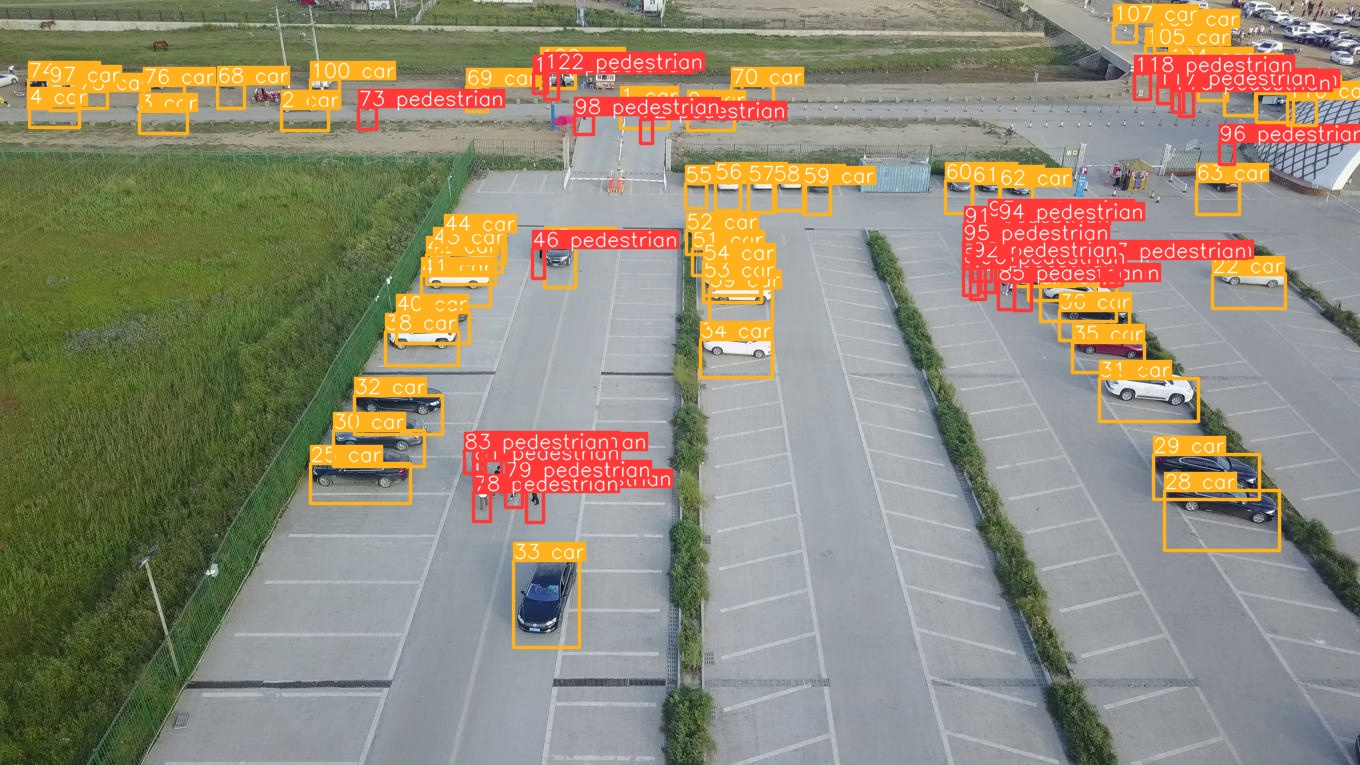
\includegraphics[width=0.85\textwidth]{11-2}
    \caption{Пример ошибок в трекинге по причине движения камеры}
    \label{img:11-2}
\end{figure}

В данном алгоритме постобработки имеется 2 управляющих параметра: $interval$ и $\tau$, первый из которых отвечает за количество кадров, участвующих в поиске объекта, а второй -- за степень сглаживания траектории. В результате экспериментов с их варьированием были получены оптимальные для данной задачи значения:

\begin{equation}
    interval = 5,
\end{equation}

\begin{equation}
    \tau = 9.
\end{equation}

В результате применения полученных значений параметров значительно уменьшилось влияние движения камеры на полученные траектории.

\subsection{Постобработка и полученные результаты}

Важно заметить, что в результате работы алгоритма трекинга StrongSORT прослеживается нестабильный характер расположения ограничивающих рамок вдоль траекторий объектов по причине движения камер беспилотных летательных аппаратов.

Для устранения данной проблемы и улучшения полученных после трекинга результатов к траекториям была применена линейная интерполяция, позволяющая восстанавливать пропадающие ограничивающие рамки объектов, а также гауссовское сглаживание, обеспечивающее плавность траекторий.

После применения вышеописанных модификаций к модели при помощи инструментов, предоставленных организаторами соревнования для датасета VisDrone, был получен $AP \ 56.45$, представленный в сравнительной Таблице \ref{tbl:12-1}.

\vspace{0.5cm}

\begin{table}[ht]
    \centering
    \begin{tblr}{c|c|c|c|c}
        \hline[1.5pt]
        Алгоритм & $AP$ & $AP_{0.25}$ & $AP_{0.5}$ & $AP_{0.75}$ \\
        \hline[1.5pt]
        SOMOT & \textbf{{\color{myred}58.61}} & \textbf{{\color{myred}70.75}} & \textbf{{\color{myred}61.26}} & \textbf{{\color{myred}43.84}} \\
        \hline
        YOLOv5-StrongSORT-GSI & \textbf{\color{mygreen}56.45} & \textbf{\color{mygreen}67.83} & \textbf{\color{mygreen}57.13} & \textbf{\color{myblue}42.35} \\
        \hline
        GIAOTracker-Fusion & \textbf{\color{myblue}54.18} & \textbf{\color{myblue}63.41} & \textbf{\color{myblue}55.35} & \textbf{\color{mygreen}43.78} \\
        \hline
        MMDS & 52.68 & 62.92 & 53.42 & 41.69 \\
        \hline
        Deep IoU Tracker & 48.54 & 63.16 & 48.11 & 34.33 \\
        \hline
        YOLO-DeepSORT-VisDrone & 46.70 & 57.43 & 48.92 & 33.75 \\
        \hline
        CenterPointCF & 44.03 & 56.91 & 44.09 & 31.09 \\
        \hline
        MIYoT & 39.35 & 50.72 & 39.25 & 28.10 \\
        \hline
        HNet & 24.71 & 33.88 & 24.35 & 15.89 \\
        \hline[1.5pt]
    \end{tblr}
    \caption{Сравнение полученных результатов с известными решениями}
    \label{tbl:12-1}
\end{table}

\subsection{Применение встроенных алгоритмов трекинга YOLOv8}

В YOLOv8 представлены реализованные алгоритмы трекинга, такие как BoT-SORT и ByteTrack \cite{13-1}, поддерживающие трекинг как для моделей классификации, так и для моделей сегментации.

В целях сравнения работы встроенных алгоритмов трекинга из YOLOv8 и используемого в основной работе алгоритма StrongSORT на базе YOLOv5 было проведено обучение модели YOLOv8x на стандартном датасете VisDrone длительностью в 50 эпох, показавшее результат $mAP \ 34.3$, что на $4.3$ выше, чем у YOLOv5.

На датасете с примененными к нему аугментациями точность достигла $mAP \ 49.4$, что также показывает увеличение на $1.3$ по сравнению с YOLOv5.

\vspace{0.5cm}

\begin{table}[ht]
    \centering
    \begin{tblr}{c|c|c}
        \hline[1.5pt]
        Этап & YOLOv8 $mAP$ & YOLOv5 $mAP$ \\
        \hline[1.5pt]
        Без аугментаций & 34.3 & 30.0 \\
        \hline
        С аугментациями & 49.4 & 48.1 \\
        \hline[1.5pt]
    \end{tblr}
    \caption{Сравнение результатов YOLOv5 и YOLOv8 на этапе покадрового детектирования}
    \label{tbl:13-1}
\end{table}

Однако представленные алгоритмы трекинга, уже примененные ранее при работе с YOLOv5 и показавшие результаты хуже StrongSORT, в очередной раз не смогли добиться корректной работы, показав на модели, обученной без аугментаций, $AP \ 42.5$, а на модели с аугментациями -- $AP \ 52.2$, в то время как точность StrongSORT для YOLOv5 достигла $AP \ 56.45$.

\vspace{0.5cm}

\begin{table}[ht]
    \centering
    \begin{tblr}{c|c|c}
        \hline[1.5pt]
        Этап & YOLOv8 $AP$ & YOLOv5 $AP$ \\
        \hline[1.5pt]
        С аугментациями & 52.2 & 56.45 \\
        \hline[1.5pt]
    \end{tblr}
    \caption{Сравнение результатов YOLOv5 и YOLOv8 на этапе трекинга}
    \label{tbl:13-2}
\end{table}

\subsection{Обзор существующих решений}

В статье \cite{14-1}, опубликованной по результатам соревнования VisDrone-MOT2021, представлены наилучшие решения, большинство из которых основаны на базе модели детектирования. В ведущих решениях используется множество передовых технологий, таких как Cascade R-CNN и CenterNet для детектирования объектов, а также DeepSORT, IOU и FairMOT для трекинга.

\textbf{Simple Online Multi-Object Tracker (SOMOT).} Модель детектирования основана на Cascade R-CNN, предобученной на датасете COCO, и embedding модель -- на Multiple Granularity Network (MGN) \cite{14-2}. Для этапа ассоциации построен трекинг множества объектов, использующий идеи DeepSORT и FairMOT, в начале инициализирующий множество треклетов, основываясь на полученных ограничивающих рамках первого кадра, а далее соотносящий новые рамки с треклетами в соответствии с вычисленным расстоянием между ними с учетом особенностей внешнего вида каждого треклета.

\textbf{GIAOTracker-Fusion.} Модель, состоящая из базового трекера, глобального трекера и пост-трекера. Базовая часть использует DetectoRS \cite{14-3} в качестве модели детектирования, предварительно обученную на датасете COCO и дообученную на VisDrone2019MOT, а в качестве трекера используется алгоритм DeepSORT. В целях стабилизации изображений из-за влияния движения камеры используется ORB+RANSAC, объединяющий механизм feature bank из DeepSORT, алгоритм обновления признаков из FairMOT и оптимизацию алгоритма Калмана. Также используется более мощное извлечение признаков при помощи OSNet \cite{14-4}. Глобальный трекер основан на треклетах из базового трекера, для извлечения признаков и ассоциаций которых используется модель VideoReID. Пост-трекер основан на результатах работы алгоритма глобального трекера, а также использует постобработку, такую как интерполяция и устранение шума.

\textbf{Multi-Object Tracking Approach Based on DeepSORT (MMDS).} В качестве базового детектора используется DetectoRS, а для трекинга применяется улучшенный DeepSORT. Для уменьшения влияния движения камеры используется Enhanced Correlation Coefficient Maximization, в то время как для сопоставления объектов происходит вычисление матрицы гомографии между соседними кадрами. Вместо стандартного фильтра Калмана используется Unscented Kalman Filter (UKF) для более точной оценки положений объектов во время движения. К тому же устанавливается правило, по которому отслеживаемые объекты, не совпадающие в течение $k$ кадров, не могут быть ассоциированы с объектами на текущем кадре, где значение $k$ меняется в зависимости от параметров треклетов. Последним из улучшений является то, что до применения немаксимального подавления сначала выполняется трекинг всех объектов и удаление пересекающихся траекторий.

\textbf{Deep IOU Tracker.} В качестве модели детектирования используется ансамбль нескольких моделей Cascade R-CNN, обученных при разных конфигурациях. При детектировании изображения разделяются на несколько частей для улучшения обнаружения мелких объектов. Ассоциация происходит через венгерский алгоритм, используется IoU между ограничивающими рамками вместе с косинусным сходством ReID признаков. Для решения проблемы, связанной с движением камеры, применяется Enhanced Correlation Coefficient Maximization.

\textbf{Implementation of DeepSORT with Scaled-YOLOv4 for Visual Drone Multi-Object Tracking (YOLO-DeepSORT-VisDrone).} В основе модели детектирования лежит улучшенная версия YOLOv4 -- Scaled-YOLOv4, предобученная на датасете COCO и обученная на VisDrone2021DET. Для трекинга используется DeepSORT.

\textbf{High-Speed Online Multi-Class Multi-Object Tracking with Center Point Based Cascaded Filtering (CenterPointCF).} Для достижения высокой скорости работы при одновременном трекинге объектов всех классов используется информация о центральных точках расположений объектов и оценке точности детектора CenterNET \cite{14-5}. Для построения легковесной модели состояний объектов используется фильтр Gaussian Mixture Probability Hypothesis Density (GMPHD) \cite{14-6}, являющийся решением для рекурсивной байесовской фильтрации.

\textbf{Medianflow-IoU-YOLO-Tracker (MIYoT).} Из соображений того, что эффективность модели детектирования значительно влияет на результативность трекинга, используется одна из последних моделей детектирования YOLO наряду с IoU и визуальным трекером. Изначально выполняется процесс ассоциации на основе IoU и активируется визуальный трекер для отслеживания объектов с предыдущих кадров, которые не были сопоставлены ни с одним объектом до этого. В течение этого процесса трекинг возвращается от визуального трекера к IoU алгоритму, если обнаруживается подходящее совпадение с одним из тех объектов, которые не были найдены ранее.

\textbf{HNet.} \cite{14-7} Подход основан на идее совместного детектирования и отслеживания объектов. Метод использует обнаружение центра и предсказание смещения центра при движении. Вдохновлен CenterTrack, однако в отличие от него применяется другой процесс построения тепловой карты, использующий метод селективной реконструкции центра. Модель принимает на вход предыдущий и текущий кадры, а также заранее преобразованную версию тепловой карты предыдущего кадра. На выходе получается тепловая карта, содержащая два гауссовских пика, представляющих местоположения центров. Наряду с этим модель предсказывает ограничивающие рамки и вектор движения для каждого объекта.

\section*{Заключение}
\addcontentsline{toc}{section}{Заключение}

По сей день задача отслеживания объектов на фото- и видеоматериалах, полученных с беспилотных летательных аппаратов, остается одной из наиболее трудоемких областей применения нейросетевых алгоритмов. Несмотря на множество недавних исследований, подвигнутых появлением обширных датасетов и соревнований соответствующей тематики, существующие модели все еще имеют значительные ограничения и не позволяют решать поставленную задачу в полной мере.

В случае дальнейших исследований в направлении отслеживания объектов вызывает интерес вопрос о межкамерном трекинге \cite{16-1}, используемом для построения траектории объекта по нескольким камерам видеонаблюдения, которые имеют непересекающиеся области обзора. Адаптирование данной задачи под реалии группы беспилотных летательных аппаратов \cite{16-2} в перспективе может существенно повысить качество результатов в данной области.

\section*{Выводы}
\addcontentsline{toc}{section}{Выводы}

В данной работе была рассмотрена задача трекинга множества объектов и ее решения, реализована обработка датасетов VisDrone и UAVDT, решившая проблему несбалансированности классов, и представлена модель, состоящая из модели детектирования YOLOv5, алгоритма трекинга StrongSORT и алгоритма постобработки GSI.

Полученная модель, предоставляющая точность $AP \ 56.45$, становится конкурентноспособной наряду с рассмотренными существующими решениями благодаря высокой точности среди достигаемых на данный момент, легковесности и высокой скорости работы, а также обходит встроенные алгоритмы трекинга модели YOLOv8.


\cleardoublepage
\phantomsection
\addcontentsline{toc}{section}{Список литературы}

\bibliographystyle{IEEEtran}
\bibliography{refs}

\end{document}
